\chapter{Exact solution for Lens Models}

\section{Axially-Symmetric Models}

Include general description for this kind of models

\subsection{SIS}
The most single lens model for galaxies  corresponds to Singular Isothermal
Sphere. This model, is obtained by assuming a spherical mass distribution
that behaves as an isothermal gas in hidrostatic equilibrium. In this case,
the density is given by

\begin{equation}
 \rho(r)=\dfrac{\sigma_v^2}{2\pi G r^2},
\end{equation}
where $\sigma_v$ is the peculiar velocity  and $r=\sqrt{\xi^2+z^2}$ is the
distance to the center of the sphere. 

Choosing $\xi_0= \dfrac{4\pi \sigma^2_v D_{\rm LS} D_{\rm OS}}{c^2 D_{\rm
OS}}$ for the dimensionless coordinates $\vec{x}=\frac{\vec{\xi}}{\xi_0}$, the
lensing potential is given by

\begin{equation}
 \varphi(x)=x,
\label{sis_pot}
\end{equation}
where $x=\sqrt{x^2_1+x^2_2}$. From the lensing potential above, the lensing
functions are
\begin{eqnarray}
 \alpha(\vec{x}) &=& 1 \label{sis_angle}\\
\kappa(\vec{x}) &= & \dfrac{1}{2x} \label{sis_convg}\\
\gamma(\vec{x}) & = &  \dfrac{1}{2x} \label{sis_shear}.
\end{eqnarray}
Notice that, the vectorial expression for the deflection angle,
Eq.~(\ref{sis_angle}), is
\begin{equation}
 \vec{\alpha}(\vec{x})=\cos{\phi}\hat{\imath} + \sin{\phi}\hat{\jmath},
\end{equation}
where $\phi=\arctan{(x_2/x_1)}$.

For this model, the eigenvalues of the Jacobian matrix of lens mapping are:
\begin{eqnarray}
\lambda_r(x)&=&1 \label{lr_sis}\\
\lambda_t(x)&=&1-\dfrac{1}{x} \label{lt_sis}.
\end{eqnarray}

This is, the SIS model does not produce image elongated in the radial direction, therefore $x_{rcc}=0$ (the radial critical curve is degenerated into a point). The parametric equation of the radial caustic is
\begin{equation}
y_{1{\rm rca}}=-\cos{\phi}, \quad y_{2{\rm rca}}-\sin{\phi} \qquad \textrm{where\ } 0\leq \phi \leq 2\pi 
\end{equation}

However, the SIS produces images elongated in the tangential direction. The tangential critical curve is a circle of radius $x_{\rm tcc}=1$ (in dimension coordinates is a circle with radius $R_{\rm E}$). Then the parametric equation of the tangential critical curve is
\begin{equation}
x_{1{\rm tcc}}=x_{\rm tcc}\cos{\phi}, \quad x_{2{\rm tcc}}=x_{\rm tcc}\sin{\phi} \qquad \textrm{where\ } 0\leq \phi \leq 2\pi 
\end{equation}
And the tangential caustic is degenerated into a point, i.e.,
\begin{equation}
y_{1{\rm tca}}=0, \quad y_{2{\rm tcc}}=0 
\end{equation}

\subsection{NFW}

\section{Pseudo-Elliptical Models}
To distort a circular lensing potential $\varphi(x)$ into a elliptical shape $\varphi_\varepsilon(x)$, its radial
coordinate $x$ is replaced by $x_\varepsilon$, where $x_\varepsilon$ is given 
\begin{equation}
 x \rightarrow x_\varepsilon = \sqrt{x^2_{1\varepsilon}+x^2_{2\varepsilon}}=
\sqrt{a_{1\varepsilon}\,x^2_1+a_{2\varepsilon}\,x^2_2}.%
\label{subti-ellip}
\end{equation}

\noindent In general, for any choice of $a_{1\varepsilon}$ and
$a_{2\varepsilon}$, the lensing functions have simple analytical expressions.
For example, the angle deflection, convergence and the components of the
shear are 
\begin{eqnarray}
\vec{\alpha}_\varepsilon(\vec{x})&=&\alpha(x_\varepsilon)(\sqrt{a_{1\varepsilon}
} \cos { \phi_ \varepsilon},\sqrt{a_{2\varepsilon}}\sin{\phi_\varepsilon})
\label{ang_def_pe}\\
\kappa_\varepsilon(\vec{x})&=&\mathcal{A}(\varepsilon)\kappa(x_\varepsilon)
-\mathcal{B}(\varepsilon)\gamma(x_\varepsilon)\cos{2\phi_\varepsilon}
\label{kappa_pe}\\
\gamma_{1\varepsilon}(\vec{x})& = &
\mathcal{B}(\varepsilon)\kappa(x_\varepsilon)-\mathcal{A}
(\varepsilon)\gamma(x_\varepsilon)\cos{2\phi_\varepsilon} \\
\gamma_{2\varepsilon}(\vec{x})& =
&-\sqrt{\mathcal{A}^2(\varepsilon)-\mathcal{B}^2(\varepsilon)}
\gamma(x_\varepsilon)\sin{ 2\phi_\varepsilon}\\
\gamma^2_\varepsilon(\vec{x}) & = &
\mathcal{A}^2(\varepsilon)\gamma^2(x_\varepsilon)-2\mathcal{A}
(\varepsilon)\mathcal {B}
(\varepsilon)\kappa(x_\varepsilon)\gamma(x_\varepsilon)\cos{2\phi_\varepsilon}
\nonumber  \\ &  &
+\mathcal{B}^2(\varepsilon)[\kappa^2(x_\varepsilon)-\sin^2{2\phi_\varepsilon}
\gamma^2(x_\varepsilon) ]\label{gamma_pe}
\end{eqnarray}
\noindent where
$\phi_\varepsilon=\arctan(\frac{x_{2\varepsilon}}{x_{1\varepsilon}})$,
$\mathcal{A(\varepsilon)}=\frac{1}{2}(a_{1\varepsilon}+a_{2\varepsilon})$ and
$\mathcal{B}(\varepsilon)=\frac{1}{2}(a_{1\varepsilon}-a_{2\varepsilon})$.
$\kappa(x_\varepsilon)$
and $\gamma(x_\varepsilon)$ are respectively the convergence and shear of any
circular model, in
which $x$ was replaced by $x_\varepsilon$.


\subsection{SIEP}
For this kind of model, from Eq.~(\ref{sis_pot}) and Eq.~(\ref{subti-ellip})
the lensing potential reads
\begin{equation}
 \varphi_\varepsilon(\vec{x})=x_\varepsilon,\label{siep_pot}
\end{equation}
 and its lensing functions are
\begin{eqnarray}
\vec{\alpha}_\varepsilon(\vec{x}) & = & (\sqrt{a_{1\varepsilon}
} \cos { \phi_ \varepsilon},\sqrt{a_{2\varepsilon}}\sin{\phi_\varepsilon})\\
\kappa_\varepsilon(\vec{x}) & = &
\left[\mathcal{A}(\varepsilon)-\mathcal{B}(\varepsilon)\cos{2\phi_\varepsilon}
\right](2 x_\varepsilon)^{-1}=\gamma_\varepsilon(\vec{x})
\end{eqnarray}
From the equations above, the components of the lens equation are
\begin{eqnarray}
 y_1&=&\dfrac{x_\varepsilon\cos{\phi_\varepsilon}}{\sqrt{a_{1\varepsilon}}}-\sqrt{a_{1\varepsilon}}\cos{\phi_ \varepsilon} \label{y1_siep}\\
y_2&=&\dfrac{x_\varepsilon\sin{\phi_\varepsilon}}{\sqrt{a_{2\varepsilon}}}-\sqrt{a_{2\varepsilon}}\sin{\phi_ \varepsilon} \label{y2_siep},
\end{eqnarray}
and the expression for the eigenvalues read
\begin{eqnarray}
\lambda_r(\vec{x})&=& 1-\kappa_\varepsilon(\vec{x})+\gamma_\varepsilon(\vec{x} )=1 \label{lr_siep}\\
\lambda_t(\vec{x})& =& 1-\kappa_\varepsilon(\vec{x})-\gamma_\varepsilon(\vec{x}
)=1-\left[\mathcal{A}(\varepsilon)-\mathcal{B}(\varepsilon)\cos{2\phi_\varepsilon } \right](x_\varepsilon)^{-1} \label{lt_siep}
\end{eqnarray}

From the Eq.~(\ref{lr_siep}) since $\lambda_r=1$ is not null, the radial critical curve is degenerated into a point $x_{rcc}=0$, and therefore the components of the radial caustic is
 \begin{eqnarray}
y_{1,rca} &=&-\sqrt{a_{1\varepsilon}}\cos{\phi_ \varepsilon}\\
y_{2,rca} &=&-\sqrt{a_{2\varepsilon}}\sin{\phi_ \varepsilon},
\end{eqnarray}

From the Eq.~(\ref{lt_siep}) the pseudo-elliptical radial coordinate of the tangential critical curve  ($\lambda_t=0$) is
\begin{equation}
x_{\varepsilon,tcc}= \mathcal{A}(\varepsilon)-\mathcal{B}(\varepsilon)\cos{2\phi_\varepsilon}, 
\end{equation}
then, the cartesian coordinates of the tangential critical are
\begin{equation}
x_{1,tcc}=\dfrac{x_{\varepsilon,tcc}\cos{\phi_\varepsilon}}{\sqrt{a_{1\varepsilon}}},\qquad x_{2,tcc}=\dfrac{x_{\varepsilon,tcc}\sin{\phi_\varepsilon}}{\sqrt{a_{2\varepsilon}}},
\end{equation}
and the componente of the tangential caustic are
\begin{eqnarray}
y_{1,tca} &=&x_{1,tcc}-\sqrt{a_{1\varepsilon}}\cos{\phi_\varepsilon}\\
y_{2,tca} &=&x_{2,tcc}-\sqrt{a_{2\varepsilon}}\sin{\phi_\varepsilon},
\end{eqnarray}

Besides, the local approximation for the length-to-width ratio of arcs $R_\lambda:=\lambda_r/\lambda_t$ implies
\begin{equation}
R_{\rm th}=\dfrac{1}{1-\left[\mathcal{A}(\varepsilon)-\mathcal{B}(\varepsilon)\cos{2\phi_\varepsilon } \right](x_\varepsilon)^{-1}},
\end{equation}
and the pseudo-elliptical radial coordinates of the curves of constant distortion (in the lens plane) are
\begin{equation}
x_{\varepsilon,R_{\rm th}}=x_{\varepsilon,tcc}\times\left\{\begin{array}{cc} \dfrac{|R_{\rm th}|}{|R_{\rm th}|-1}, & R_{\rm th}>0 \\ & \\
\dfrac{|R_{\rm th}|}{|R_{\rm th}|+1}, & R_{\rm th}<0 \end{array}\right.
\end{equation}
The cartesian components of the cuves of constant distortion in the source plane are given by the Eqs.~(\ref{y1_siep}) and (\ref{y2_siep}) where $x_\varepsilon$ is replaced by $x_{\varepsilon,R_{\rm th}}$.

In Fig.~\ref{siep_curves} we show an example for the main curves of the SIEP model in both planes, for $R_{\rm E}=1$, $\varepsilon=0.4$ (that corresponds to the lensing potential ellipticity by itself).

\begin{figure*}[!ht]
\resizebox{\hsize}{!}{
\subfigure{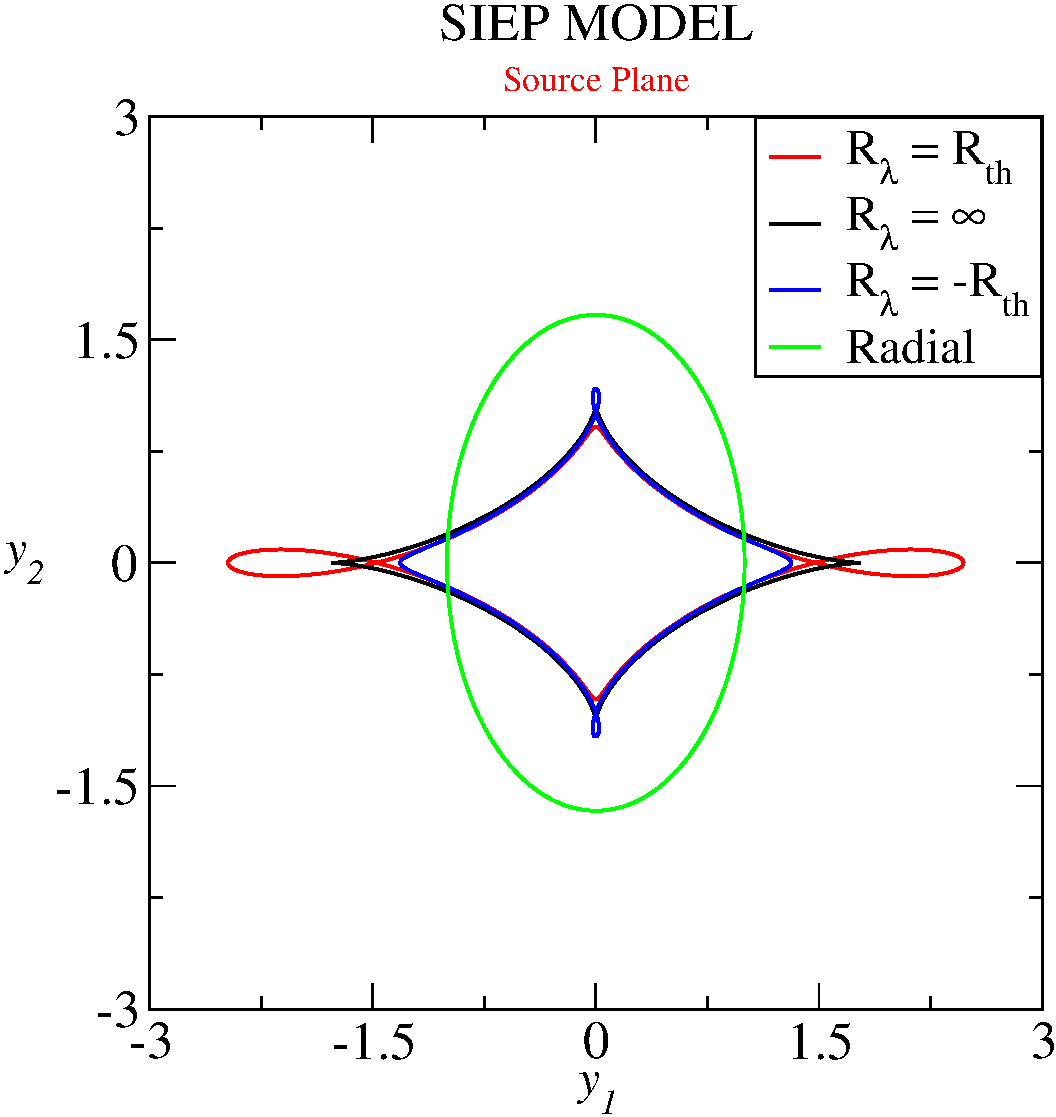
\includegraphics{graphics/siep_source_plane.pdf}}
\hspace{3.cm}
\subfigure{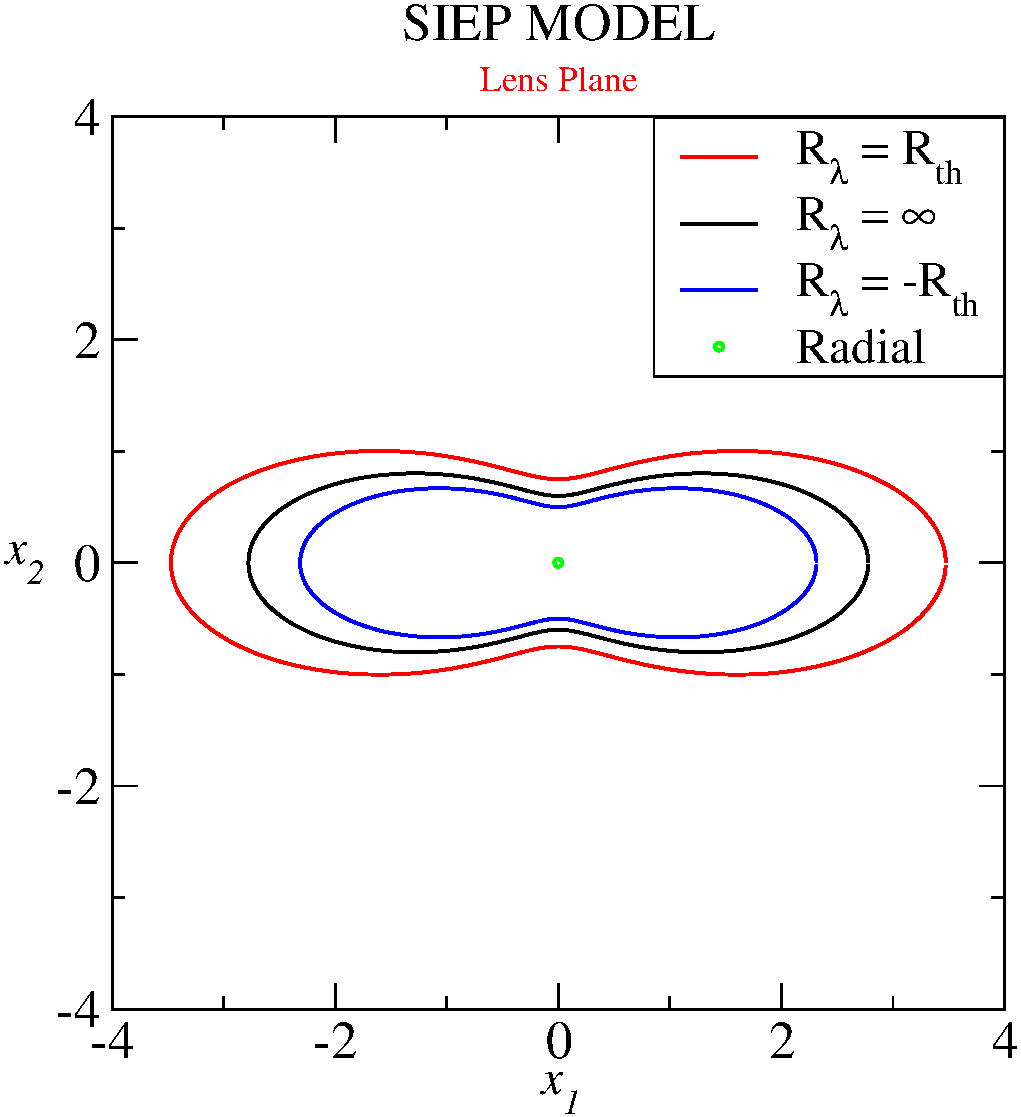
\includegraphics{graphics/siep_lens_plane.pdf}}}
\caption{\label{siep_curves}  SIEP lensing model curves. Left Panel:
Tangential ($R_\lambda=\infty$) and Radial Caustics and Curves of Constant
Distortion ($R_\lambda=\pm R_{\rm th}$) . Right Panel: Tangential
($R_\lambda=\infty$) and Radial Critical Curves and  Constant Distortion Curves
($R_\lambda=\pm R_{\rm th}$). Here, we used $R_{\rm E}=1$ and $|R_{\rm
th}|=5$ and the Keeton's parametrization,i.e,  $a_{1\varepsilon}=1$ and
$a_{2\varepsilon}=(1-\varepsilon)^{-2}$ for $\varepsilon=0.4$, }
\end{figure*}

\subsection{PNFW}
As example, we compare the result of our numerical code implemented by us,
against the solution obtained with the Gravlens Software.


\begin{figure*}[!ht]
\resizebox{\hsize}{!}{
\subfigure{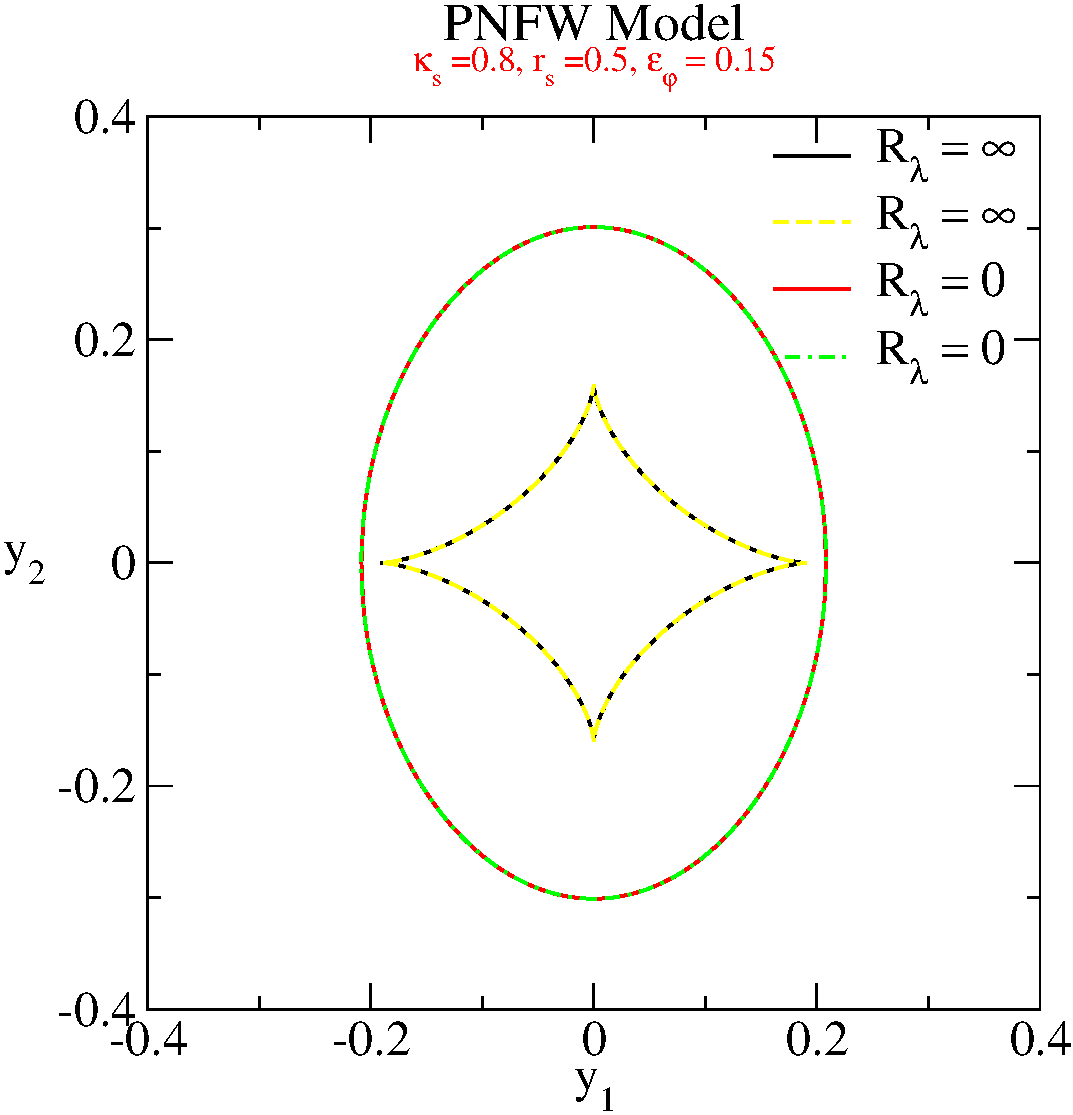
\includegraphics{graphics/compar1_src.pdf}}\hspace{3.cm}
\subfigure{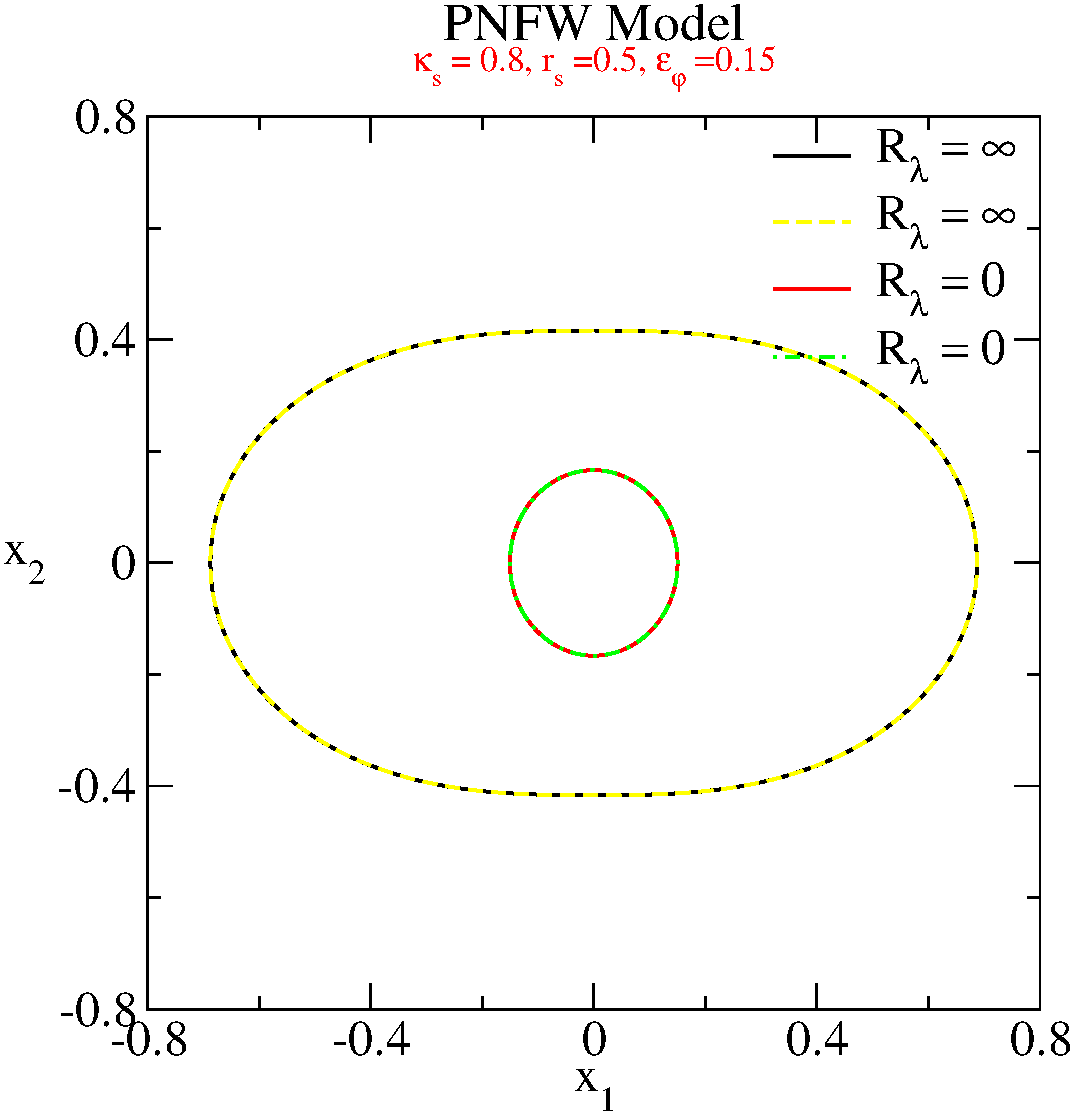
\includegraphics{graphics/compar1_lens.pdf}}}
\caption{\label{pnfw_curves1}  PNFW lensing model curves for some combination of
lens parameters. Solid lines correspond to our Fortran code and Dashed-Lines
correspond to Gravlens Software. Left Panel: Tangential and Radial Caustics.
Right Panel: Tangential and Radial Critical Curves. ($R_\lambda=\infty$:
Tangential Curves. $R_\lambda=0$: Radial Curves)}
\end{figure*}

\begin{figure*}[!ht]
\resizebox{\hsize}{!}{
\subfigure{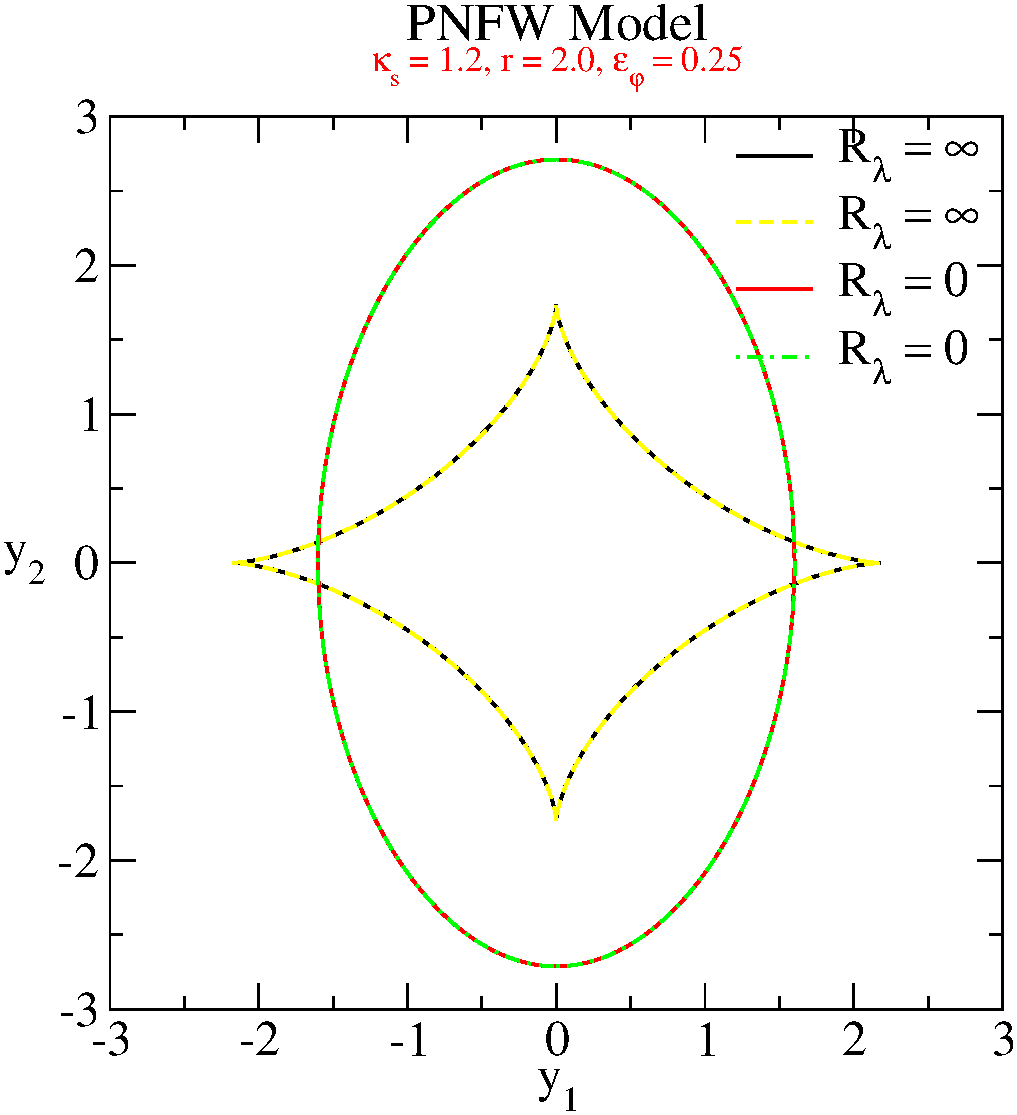
\includegraphics{graphics/compar2_src.pdf}}\hspace{3.cm}
\subfigure{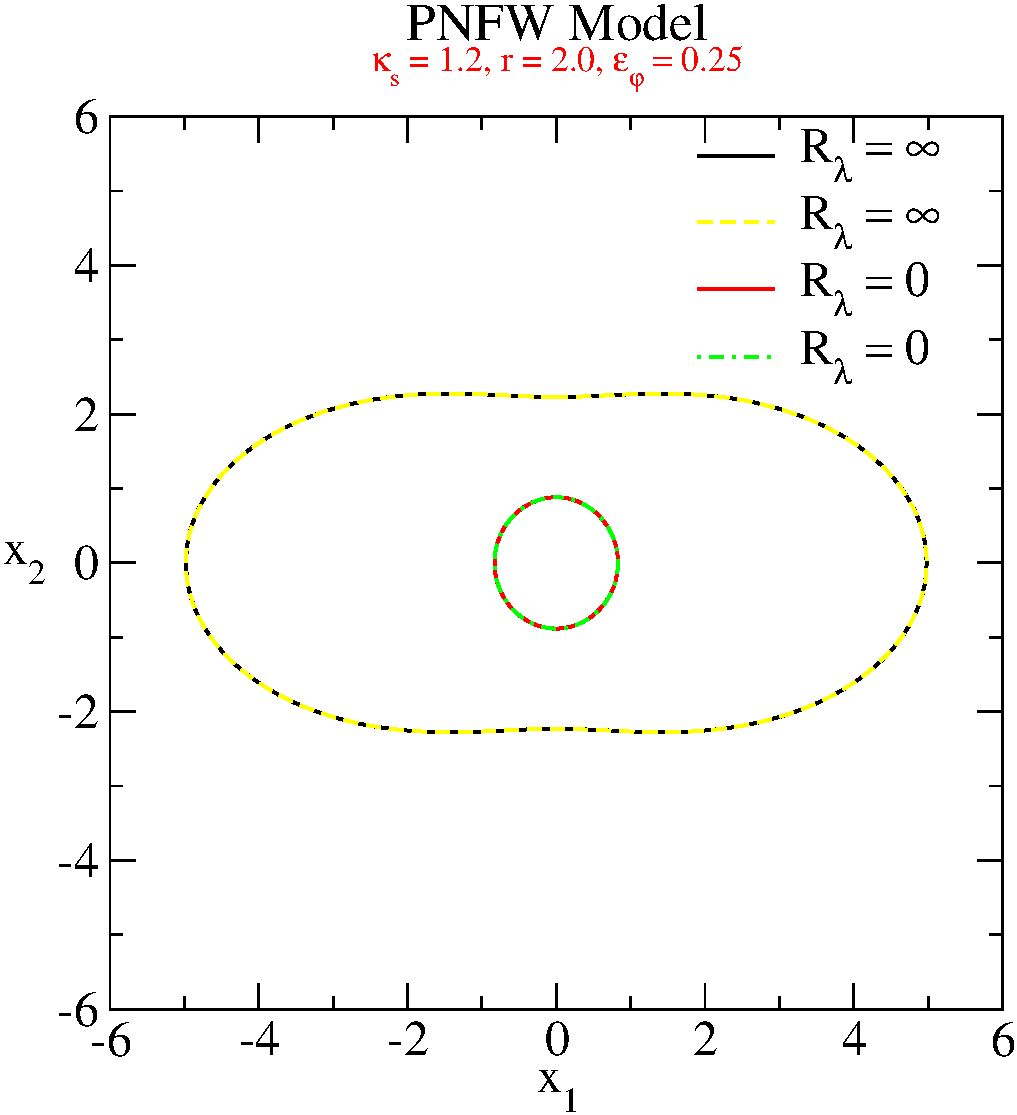
\includegraphics{graphics/compar2_lens.pdf}}}
\caption{\label{pnfw_curves2}  PNFW lensing model curves for some combination of
lens parameters. Solid lines correspond to our Fortran code and Dashed-Lines
correspond to Gravlens Software. Left Panel: Tangential and Radial Caustics.
Right Panel: Tangential and Radial Critical Curves. ($R_\lambda=\infty$:
Tangential Curves. $R_\lambda=0$: Radial Curves)}
\end{figure*}

\begin{figure*}[!ht]
\resizebox{\hsize}{!}{
\subfigure{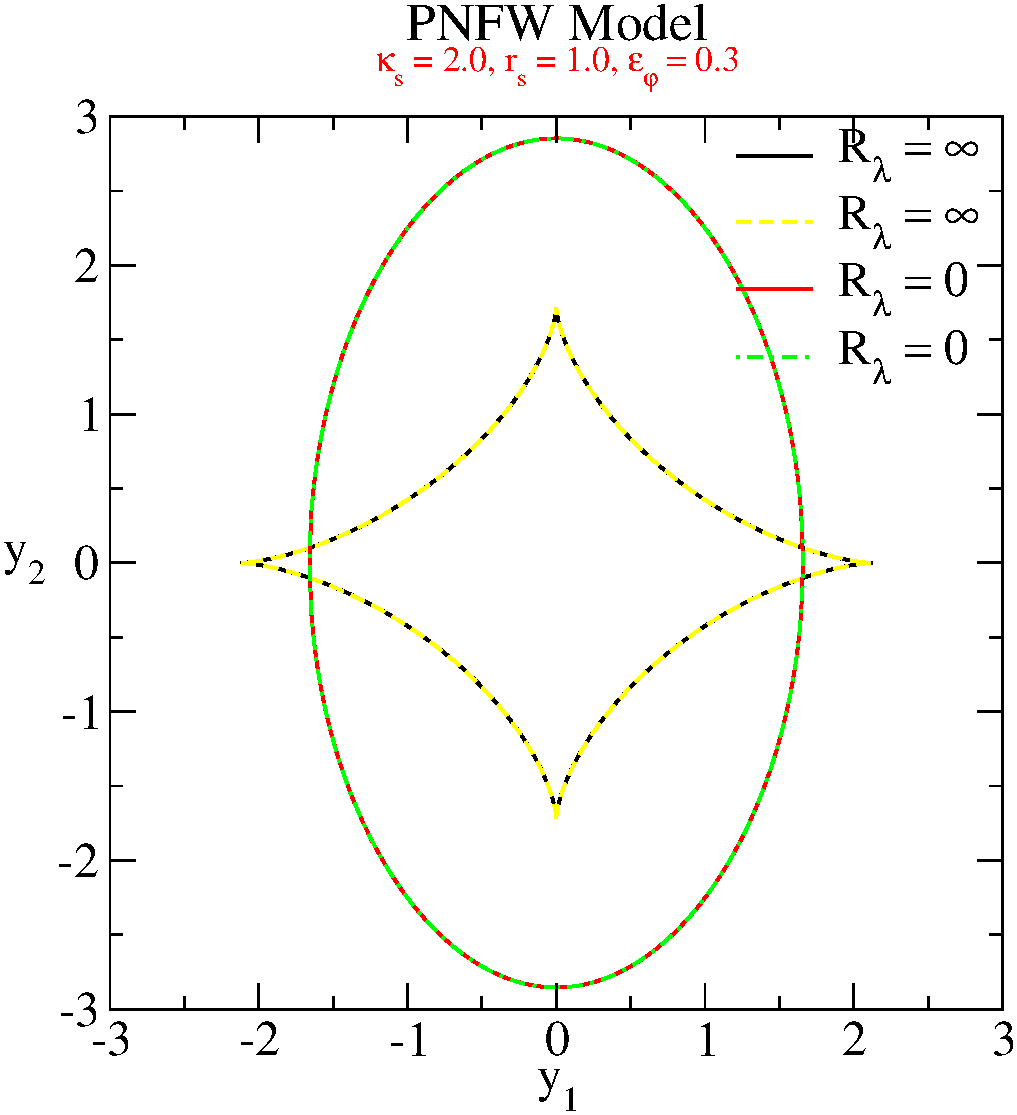
\includegraphics{graphics/compar3_src.pdf}}\hspace{3.cm}
\subfigure{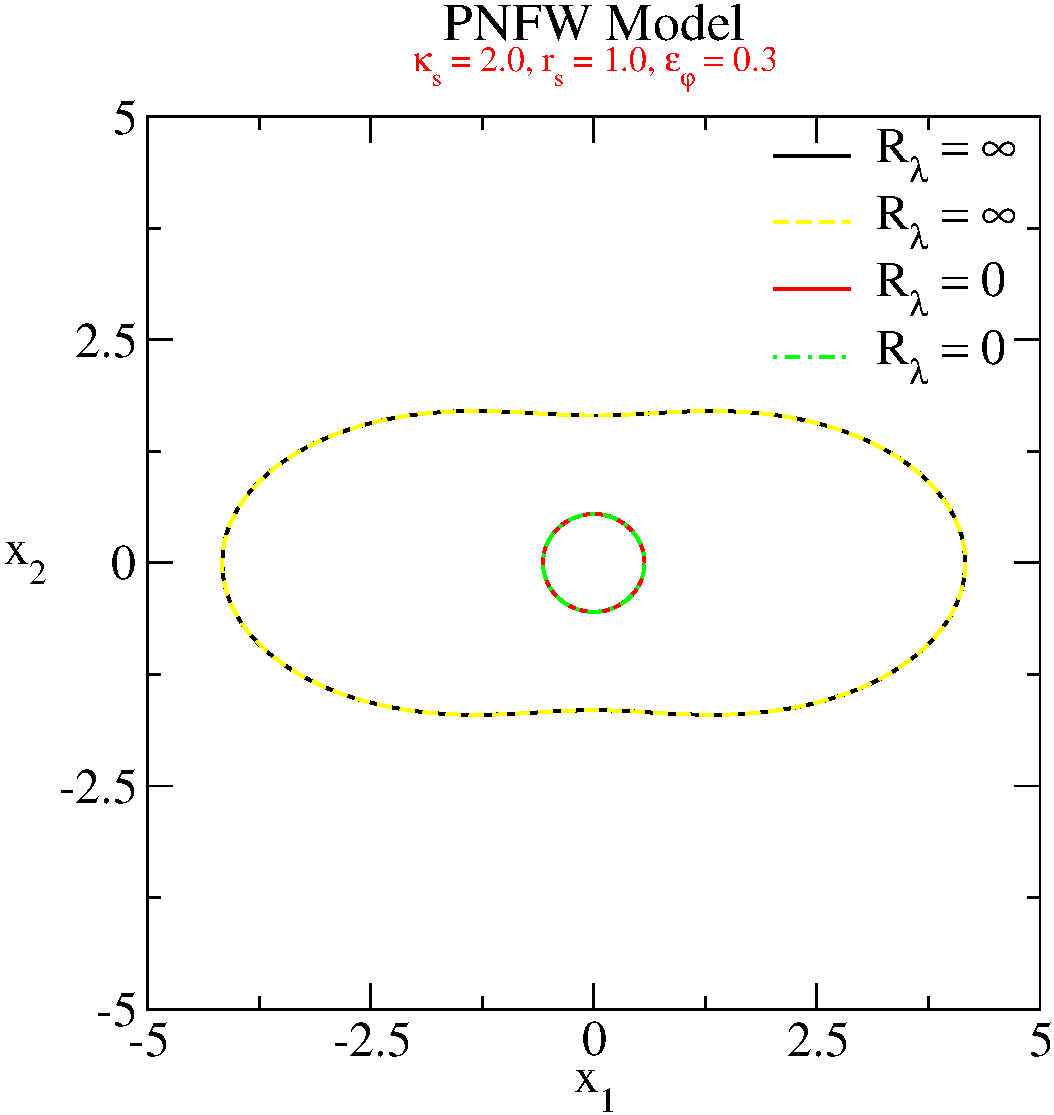
\includegraphics{graphics/compar3_lens.pdf}}}
\caption{\label{pnfw_curves3}  PNFW lensing model curves for some combination of
lens parameters. Solid lines correspond to our Fortran code and Dashed-Lines
correspond to Gravlens Software. Left Panel: Tangential and Radial Caustics.
Right Panel: Tangential and Radial Critical Curves. ($R_\lambda=\infty$:
Tangential Curves. $R_\lambda=0$: Radial Curves)}
\end{figure*}




\section{Elliptical Models}

\section{Arc Cross Section}
In this work, we compute the Arc Cross Section by using the local approximation
for the length-to-width ratio of arcs i.e., we substitute $L/W$ by 
\begin{equation}
R_\lambda:=\dfrac{\lambda_r}{\lambda_t},
\end{equation}
and the condition for minimum distortion is given by a number $R_{\rm th}$.  When we use this local measurement for the properties of the arcs, we are considering only deformation arcs and therefore, we are calculating the cross section for deformation arcs $\sigma_{\rm dcs}$

\begin{equation}
\sigma_{\rm dcs} \equiv \int d^2\eta =\int_{ \frac{\lambda_r}{\lambda_t} > |R_{\rm th}|} \left |{\rm det}\,\textbf{J}(\vec{\xi}) \right| d^2\xi.
\end{equation}

However, as we are working with dimensionless coordinates $ \vec{y}=\frac{\eta}{\eta_0}$ and $\vec{x}=\frac{\xi}{\xi_0}$ we can write $\sigma_{\rm dcs}$ as
\begin{equation}
\sigma_{\rm dcs} = \xi_0^2\tilde{\sigma}_{\rm dcs}= \xi_0^2 \int_{ \frac{\lambda_r}{\lambda_t} > |R_{\rm th}|} \left |{\rm det}\,\textbf{J}(\vec{x}) \right| d^2\!x. \label{dcs_dimensionless}
\end{equation}

In general, the calculation of this expression requires numerical method,
unless for a few kind of lens model.  For example, for the SIS model,
$\mathbf{J}(\vec{x})=1-\frac{1}{x}$, $\xi_0=\re$ and, hence we have

\begin{equation}
\sigma_{dcs}=2\pi\,R^2_{\rm E} \dfrac{|R_{\rm th}|^2+1}{(|R_{\rm th}|^2-1)^2} \label{dcs_sis}
\end{equation}

Note that the last equation is the same as the Eq.~(\ref{dcs_sis_pertapp}). The
other  model that offers an analytical expression for the cross section for
deformation arcs is the SIEP. For this model, first we have that the determinant
of the Jacobian matrix is
\begin{equation}
\mathbf{J}(\vec{x})=1-\dfrac{x_{\varepsilon,tcc}}{x_{\varepsilon}}, \label{jacob_siep}
\end{equation}
where $x_{\varepsilon,tcc}$ corresponds to the pseudo-elliptical radial
coordinate of the tangential critical curve. Then, by inserting the last
equation in Eq.~(\ref{dcs_dimensionless}), and $d^2 x=xdx d\phi$, we have

\begin{equation}
\tilde{\sigma}_{\rm siep}= \int_{0}^{2\pi}\int_{x_{_{-R_{\rm th}}}}^{x_{_{R_{\rm th}}}}\left| 1-\dfrac{x_{\varepsilon,tcc}}{x_{\varepsilon}}\right| x dx d\phi 
\end{equation}
As in polar coordinates $x_{\varepsilon}=xf(\phi)$, where $f(\phi)=\sqrt{a_{1\varepsilon}\cos^2{\phi}+a_{2\varepsilon}\sin^2{\phi}}$, the result integration in the radial coordinate is
\begin{equation}
\tilde{\sigma}_{\rm siep}= \dfrac{|R_{\rm th}|^2+1}{(|R_{\rm th}|^2-1)^2}
\int_{0}^{2\pi}\left[\mathcal{A}(\varepsilon)-\mathcal{B}(\varepsilon)\cos{
(2\phi_\varepsilon)} \right]^2 d\phi 
\end{equation}
Therefore, the analytical expression for the deformation cross section for the SIEP is
\begin{eqnarray}
\sigma_{\rm siep}&=& R^2_{\rm E}\dfrac{|R_{\rm th}|^2+1}{(|R_{\rm th}|^2-1)^2}\times \nonumber \\
& & \left\{2\pi\left[ [\mathcal{A}(\varepsilon)-\mathcal{B}(\varepsilon)]^2+\frac{2\,a_{1\varepsilon}\mathcal{B}^2(\varepsilon)}{a_{1\varepsilon}+4\,a_{2\varepsilon}\pi^{2}} \right]+ 2[2\mathcal{A}(\varepsilon)\mathcal{B}(\varepsilon)-\mathcal{B}^2(\varepsilon)]\sqrt{\frac{a_{1\varepsilon}}{a_{2\varepsilon}}}\arctan{\left( 2\pi\sqrt{\frac{a_{2\varepsilon}}{a_{1\varepsilon}}}\right)} \right\} \nonumber \\
\end{eqnarray}

In the limit $\varepsilon \rightarrow 0$, we have that $\mathcal{A}(\varepsilon)=1$, $\mathcal{B}(\varepsilon)=0$,  and the expression above is the same as Eq.~(\ref{dcs_sis}). In the Figs.~\ref{dcs_siep_re},~\ref{dcs_siep_e},~\ref{dcs_siep_rth} we show the deformation cross section for the SIEP model considering 
\begin{eqnarray}
 a_{1\varepsilon}&=&1-\varepsilon, a_{2\varepsilon}=1+\varepsilon \quad
\textrm{Angle Deflection Model} \\ 
a_{1\varepsilon} &=&1-\varepsilon,a_{2\varepsilon}=(1-\varepsilon_\varphi)^{-1} 
\quad
\textrm{Standard Parametrization} \\
a_{1\varepsilon} &=& 1, a_{2\varepsilon}=(1-\varepsilon_\varphi)^{-2}
\quad
\textrm{Keeton's Parametrization} 
\end{eqnarray}



\begin{figure*}[!ht]
\resizebox{\hsize}{!}{
\subfigure{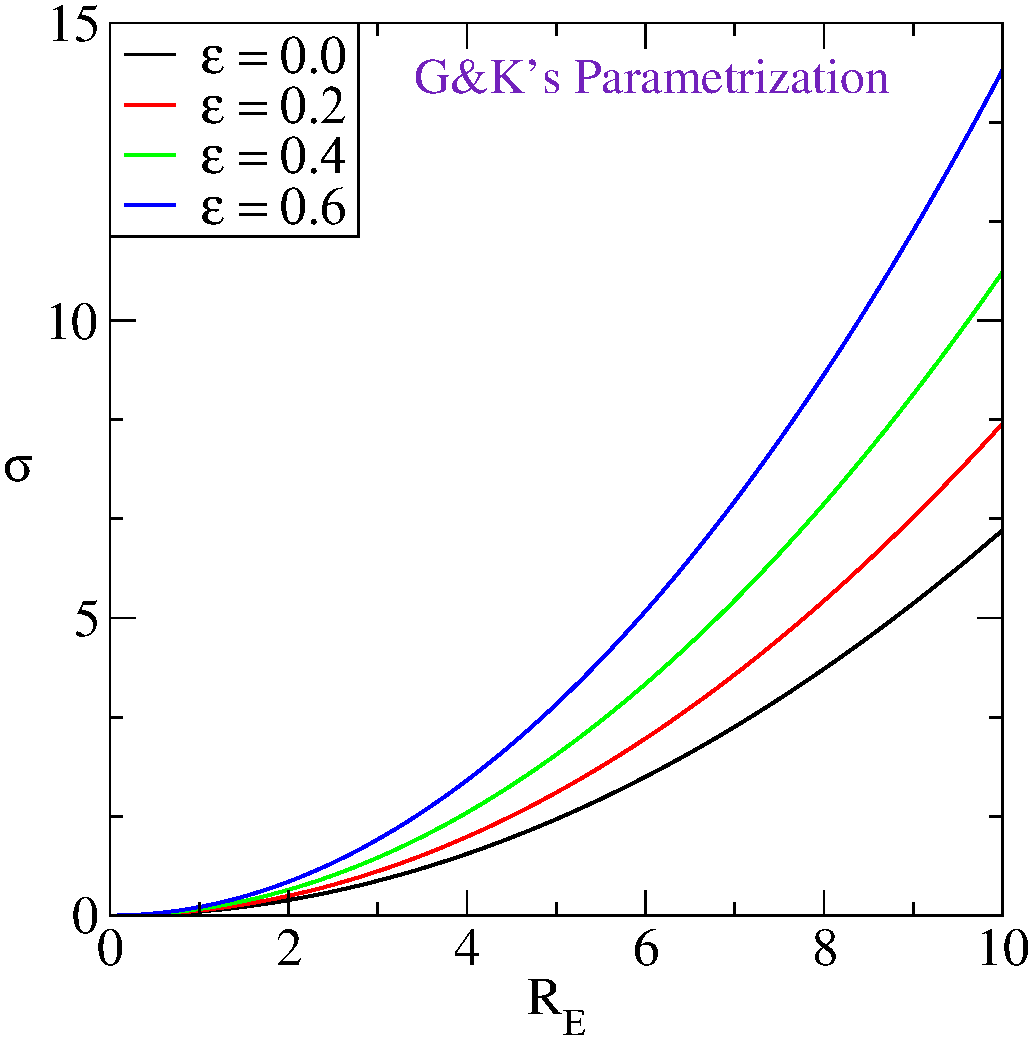
\includegraphics{graphics/dcs_siep_vs_re-gk.pdf}}\hspace{1.cm}
\subfigure{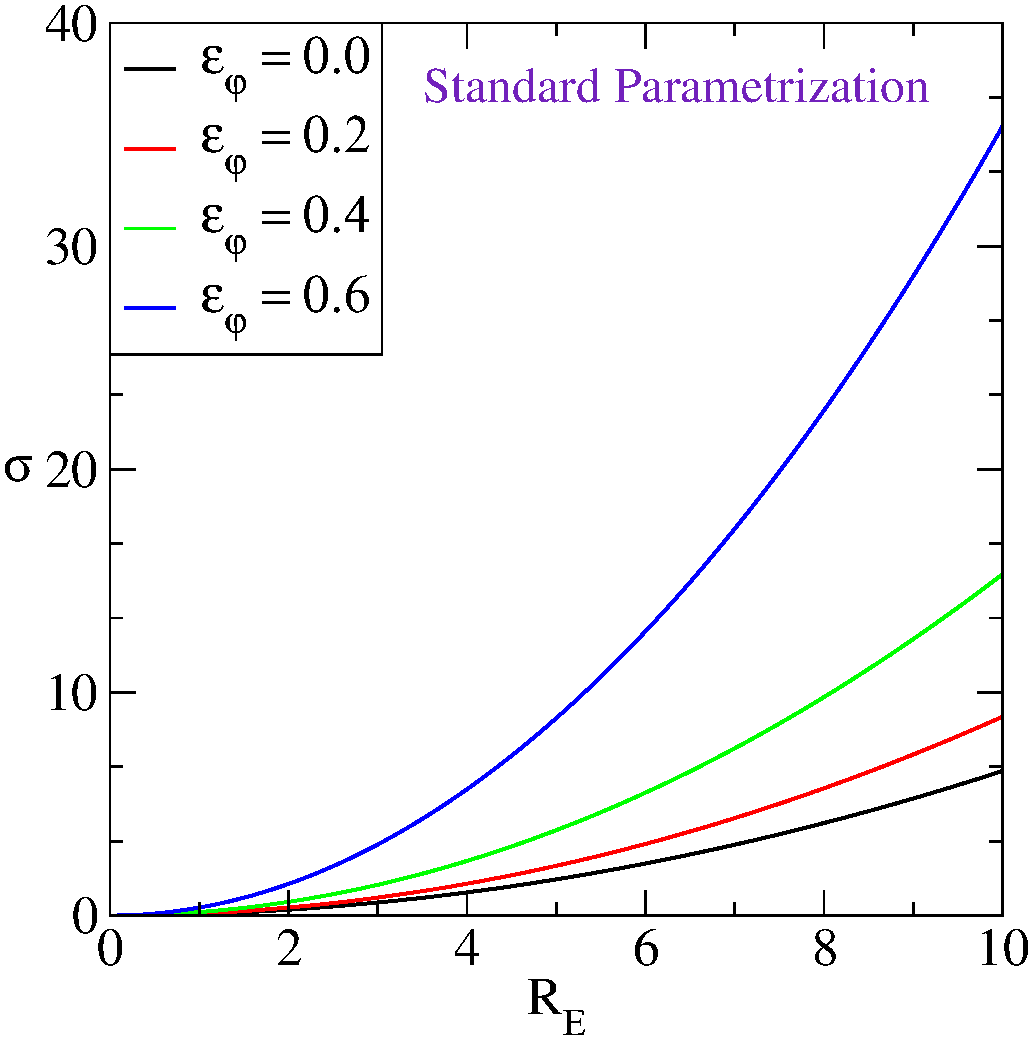
\includegraphics{graphics/dcs_siep_vs_re-st.pdf}}\hspace{1.cm}
\subfigure{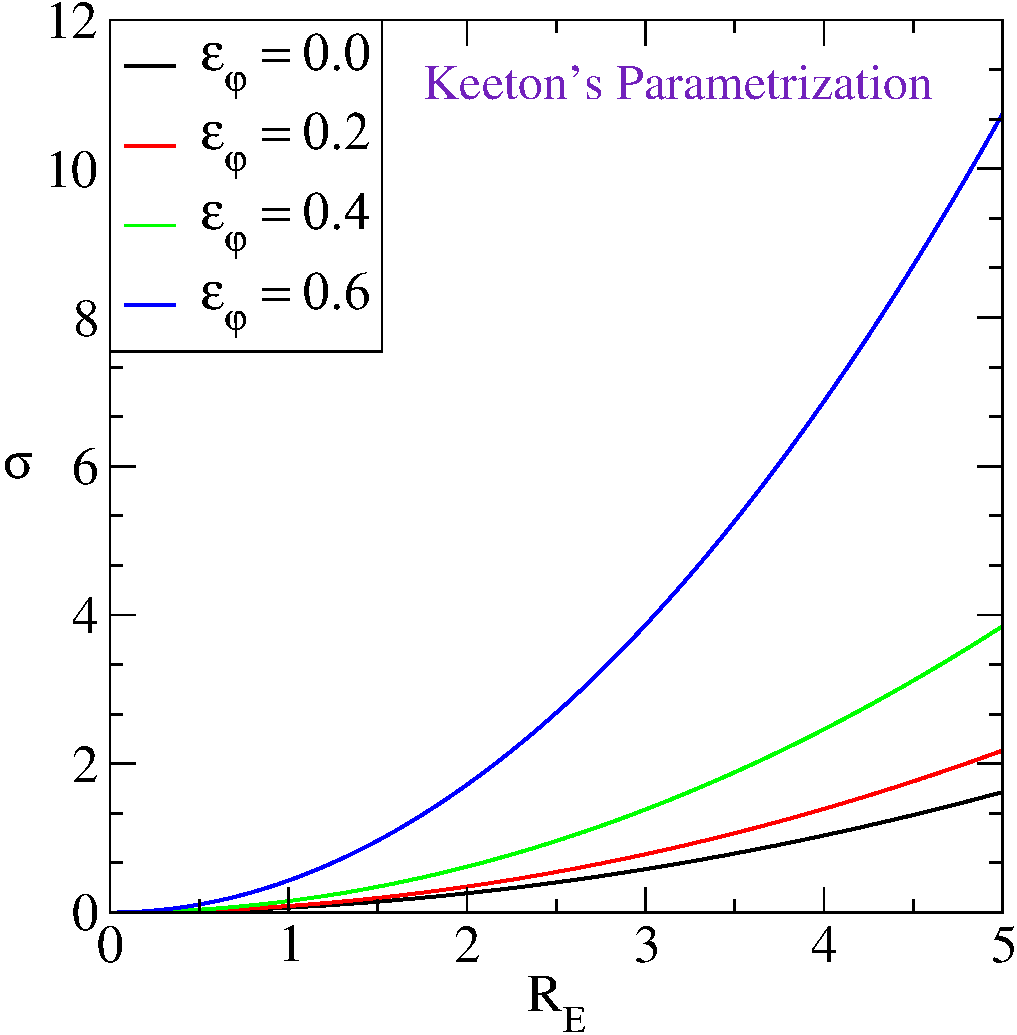
\includegraphics{graphics/dcs_siep_vs_re-k.pdf}}}
\caption{\label{dcs_siep_re} Deformation cross section for the  SIEP lensing model as a function of $R_{\rm E}$ . Left Panel:
Parametrization of the Angle Deflection Model. Middle Panel: Standard
Parametrization. Right Panel: The Keeton's parametrization.  The calculations
were done for $R_{\rm th}=10$.}
\end{figure*}

\begin{figure*}[!ht]
\resizebox{\hsize}{!}{
\subfigure{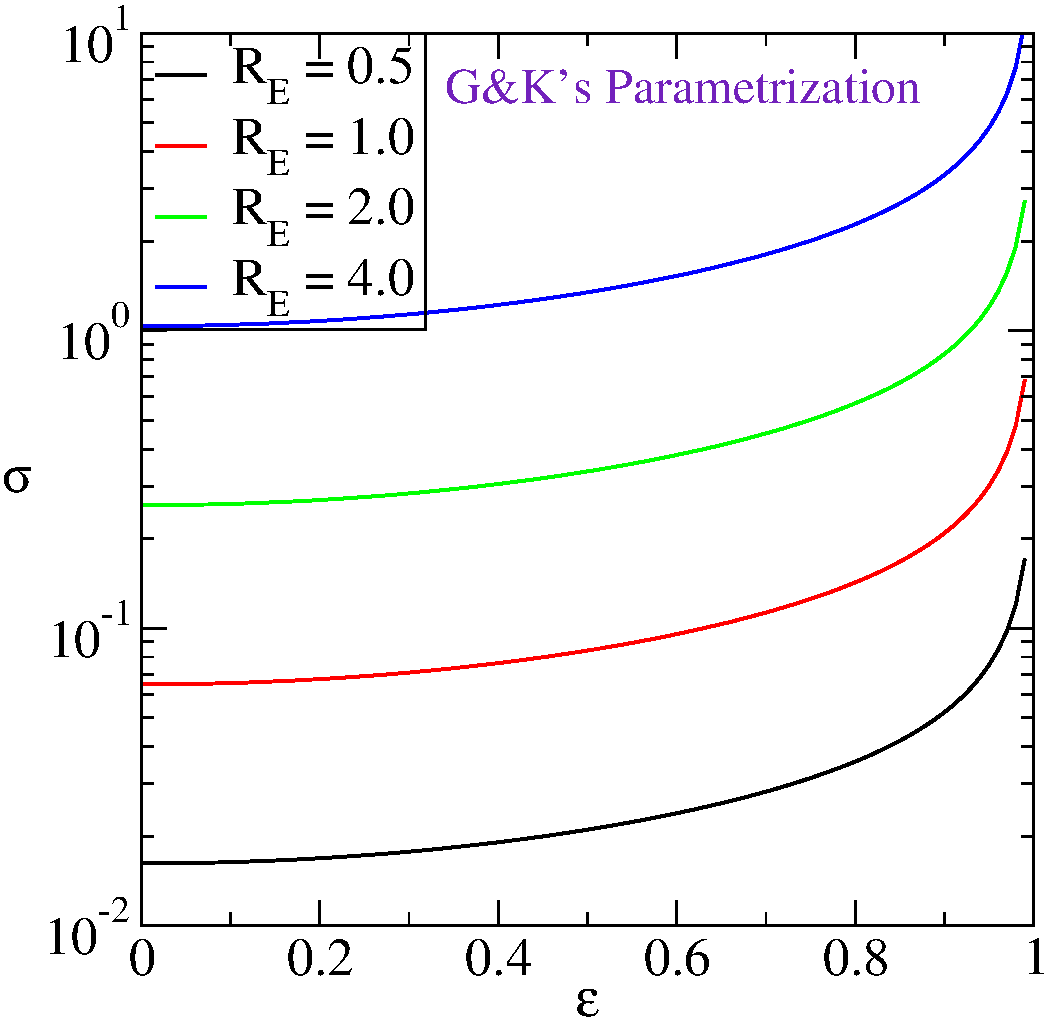
\includegraphics{graphics/dcs_siep_vs_e-gk.pdf}}\hspace{1.cm}
\subfigure{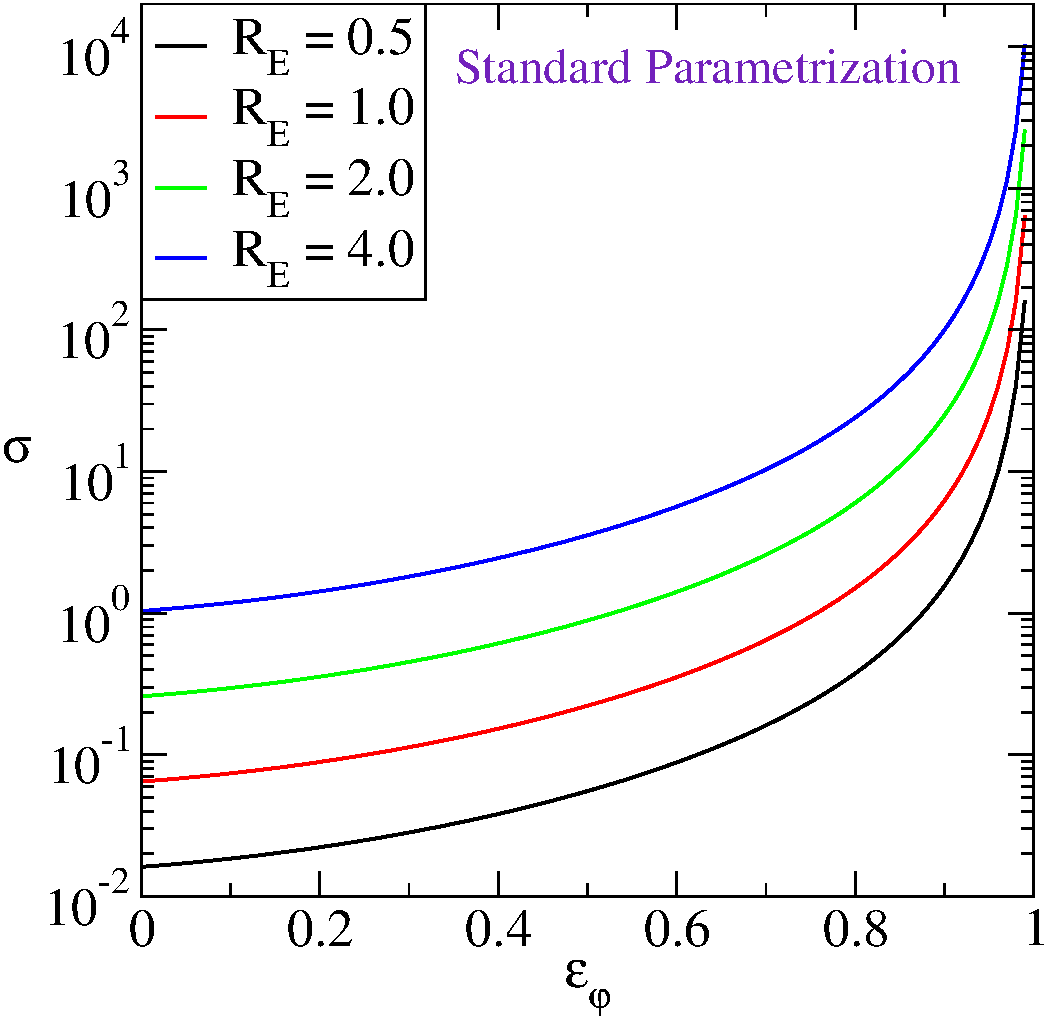
\includegraphics{graphics/dcs_siep_vs_e-st.pdf}}\hspace{1.cm}
\subfigure{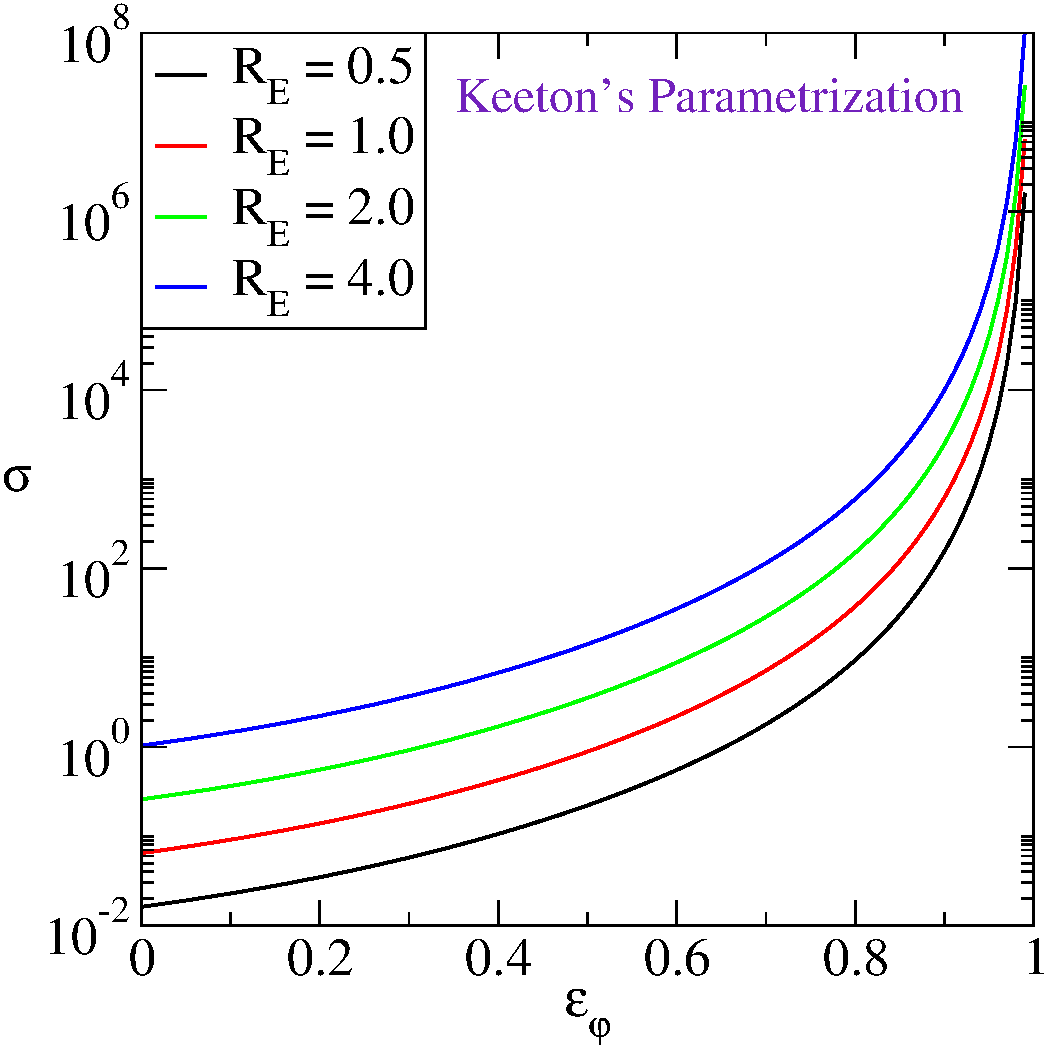
\includegraphics{graphics/dcs_siep_vs_e-k.pdf}}}
\caption{\label{dcs_siep_e} Deformation cross section for the  SIEP lensing
model as a function of the ellipticity. Left Panel:
Parametrization of the Angle Deflection Model. Middle Panel: Standard
Parametrization. Right Panel: The Keeton's parametrization. The calculations
were done for $R_{\rm th}=10$.}
\end{figure*}

\begin{figure*}[!ht]
\resizebox{\hsize}{!}{
\subfigure{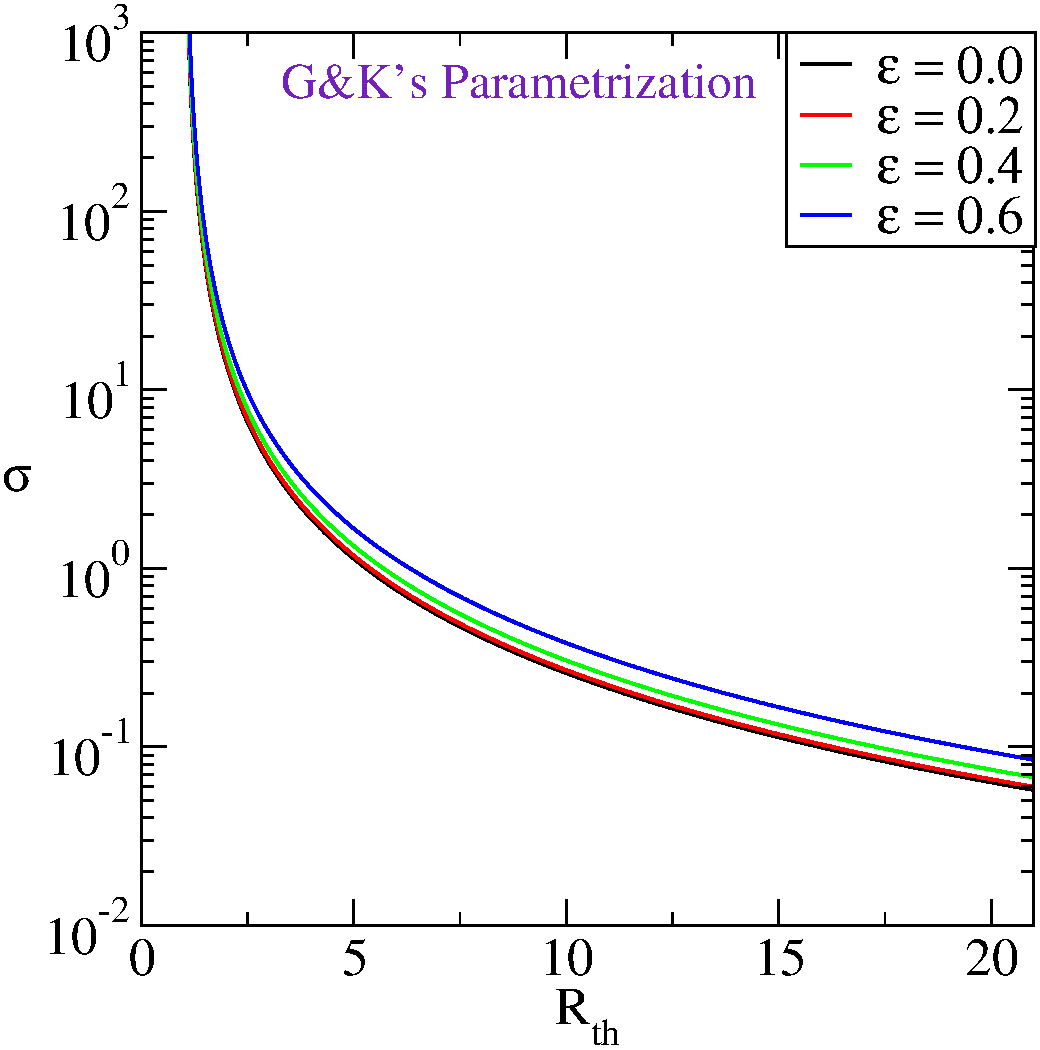
\includegraphics{graphics/dcs_siep_vs_rth-gk.pdf}}\hspace{1.cm}
\subfigure{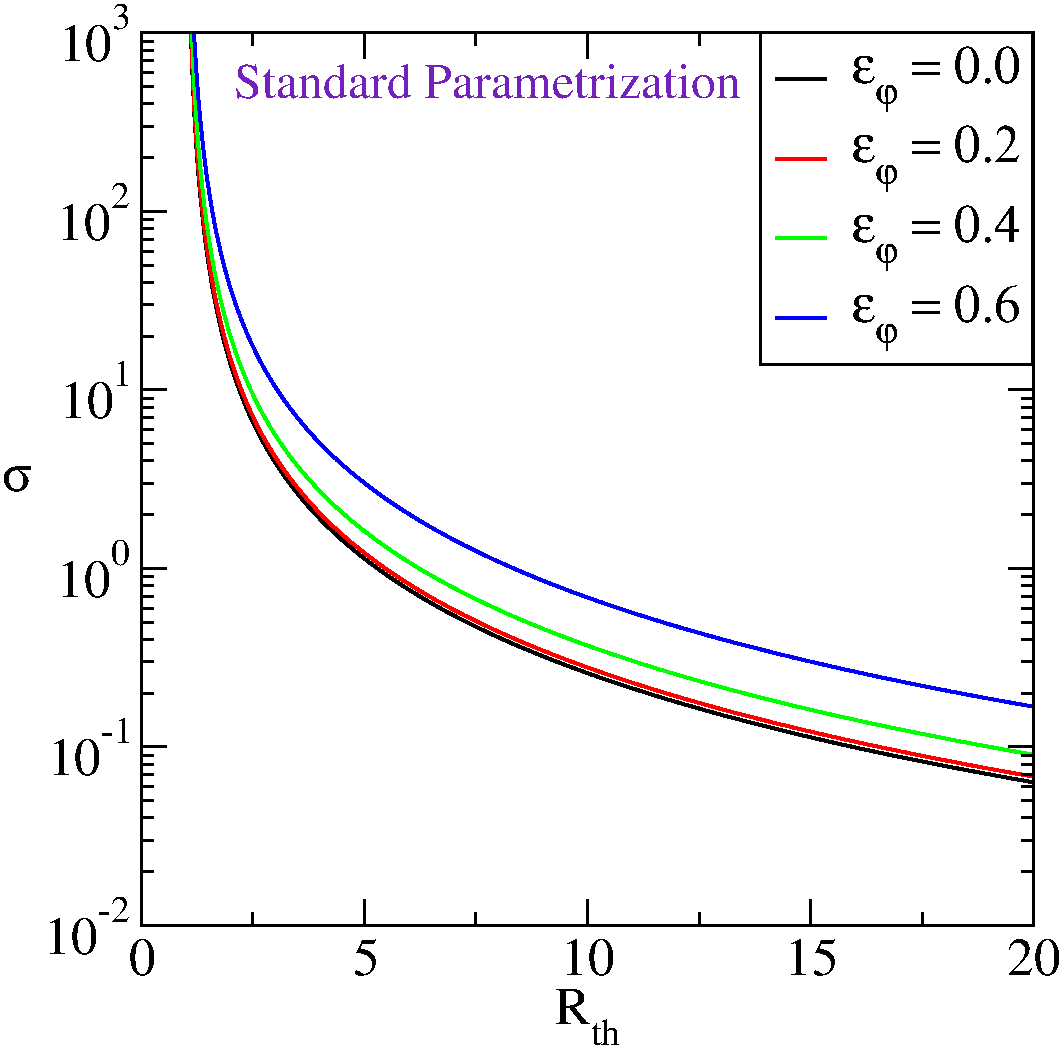
\includegraphics{graphics/dcs_siep_vs_rth-st.pdf}}\hspace{1.cm}
\subfigure{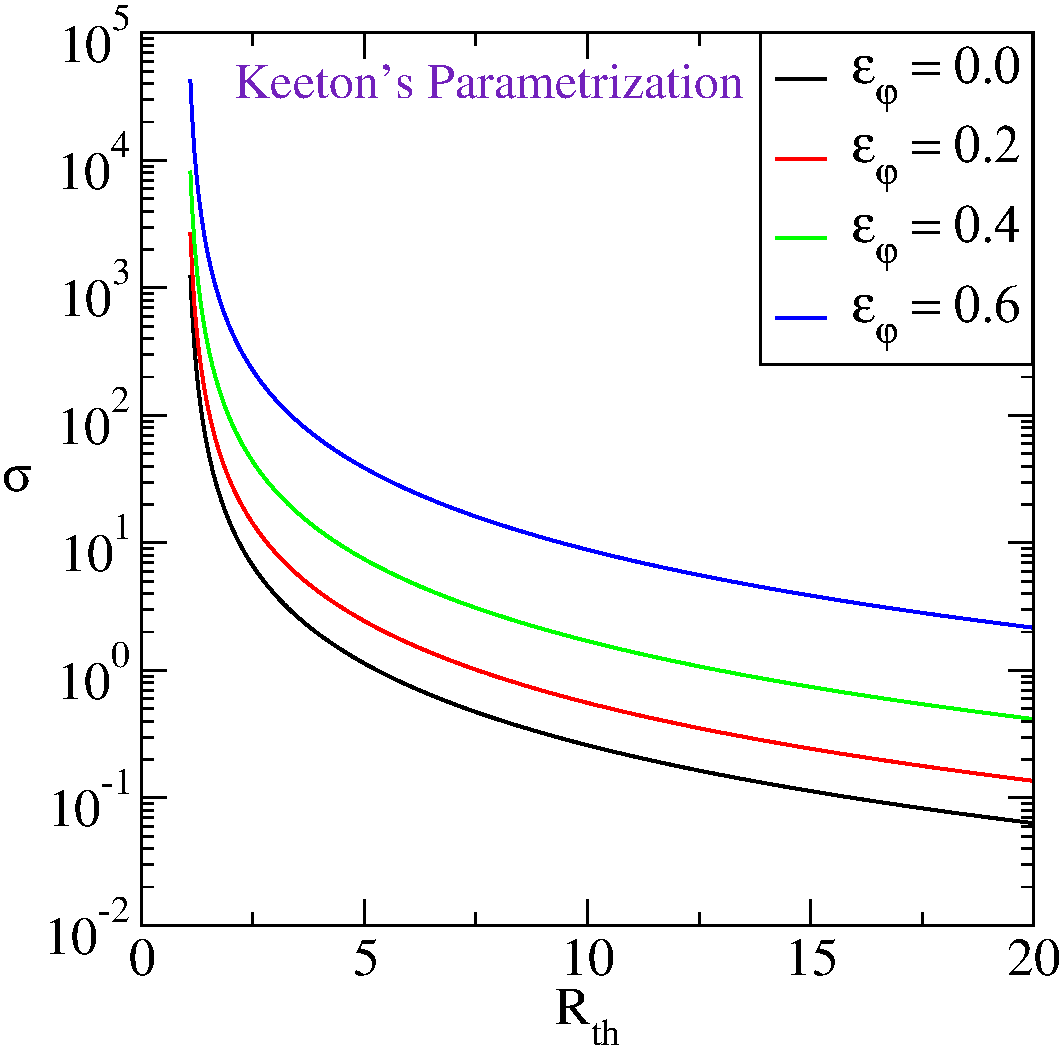
\includegraphics{graphics/dcs_siep_vs_rth-k.pdf}}}
\caption{\label{dcs_siep_rth} Deformation cross section for the  SIEP lensing
model as a function of $R_{\rm th}$. Left Panel:
Parametrization of the Angle Deflection Model. Middle Panel: Standard
Parametrization. Right Panel: The Keeton's parametrization. The calculations
were done for $R_{\rm E}=2$.}
\end{figure*}



\begin{figure*}[!ht]
\resizebox{\hsize}{!}{
\subfigure{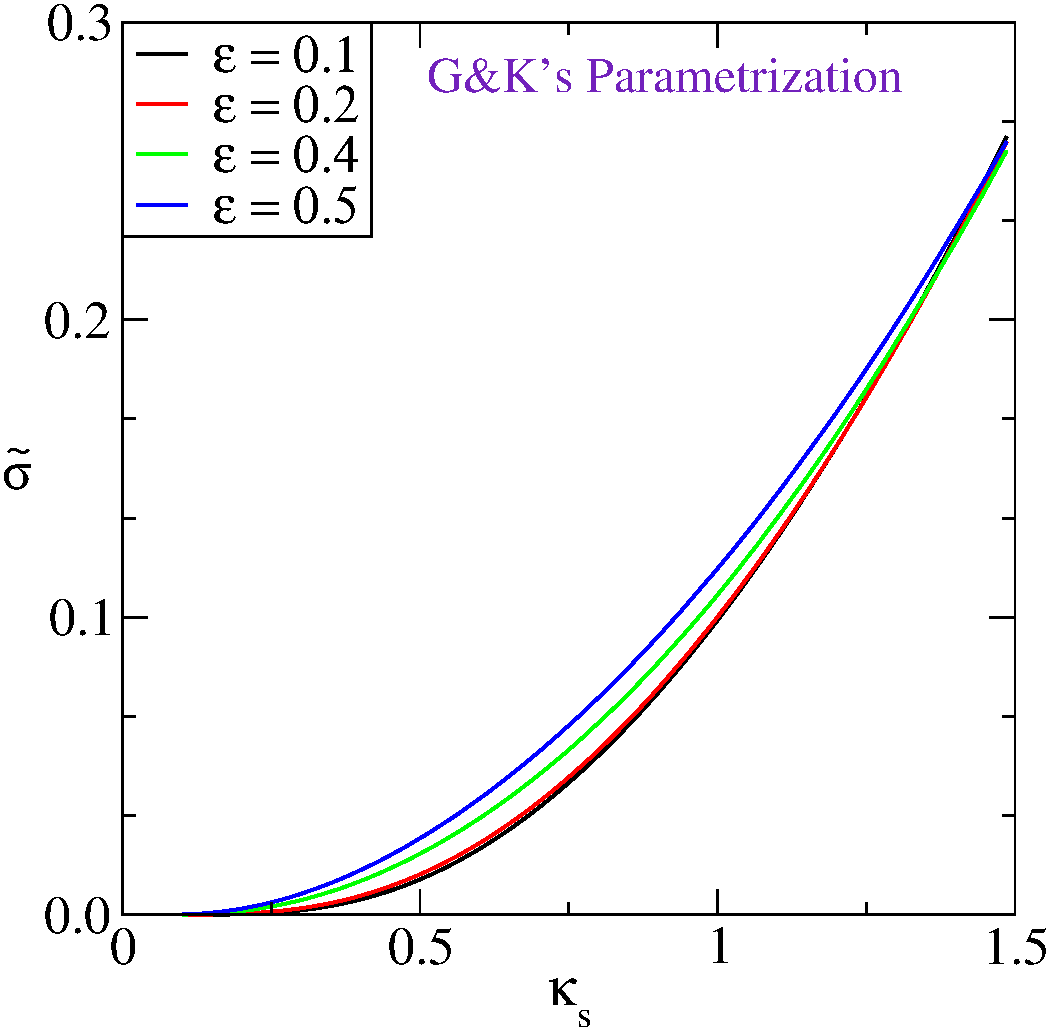
\includegraphics{graphics/dcs_pnfw_vs_ks-gk.pdf}}\hspace{1.cm}
\subfigure{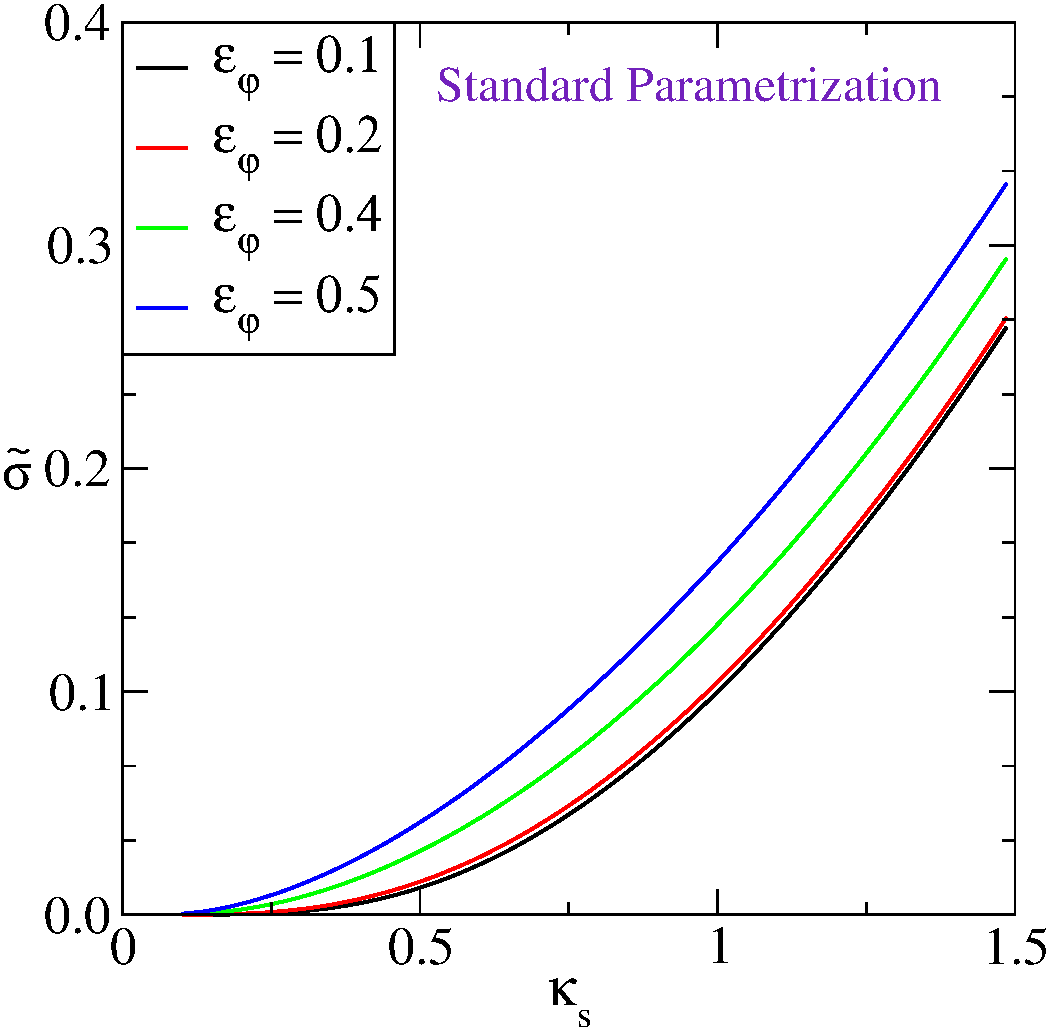
\includegraphics{graphics/dcs_pnfw_vs_ks-st.pdf}}\hspace{1.cm}
\subfigure{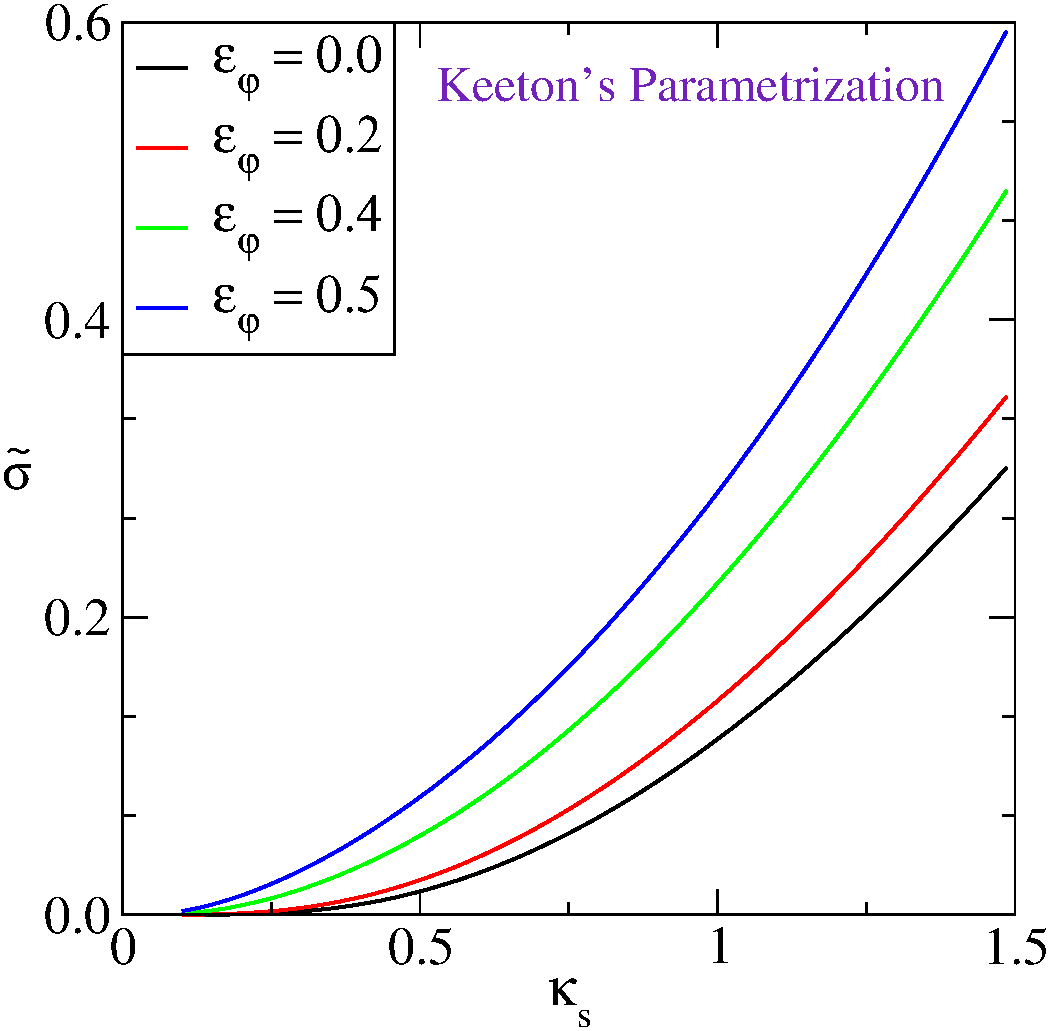
\includegraphics{graphics/dcs_pnfw_vs_ks-k.pdf}}}
\caption{\label{dcs_pnfw_ks} Deformation cross section for the  PNFW lensing
model as a function of $\kappa_s$ . Left Panel:
Parametrization of the Angle Deflection Model. Middle Panel: Standard
Parametrization. Right Panel: The Keeton's parametrization.  The calculations
were done for $R_{\rm th}=10$ and $r_s=1$.}
\end{figure*}

\begin{figure*}[!ht]
\resizebox{\hsize}{!}{
\subfigure{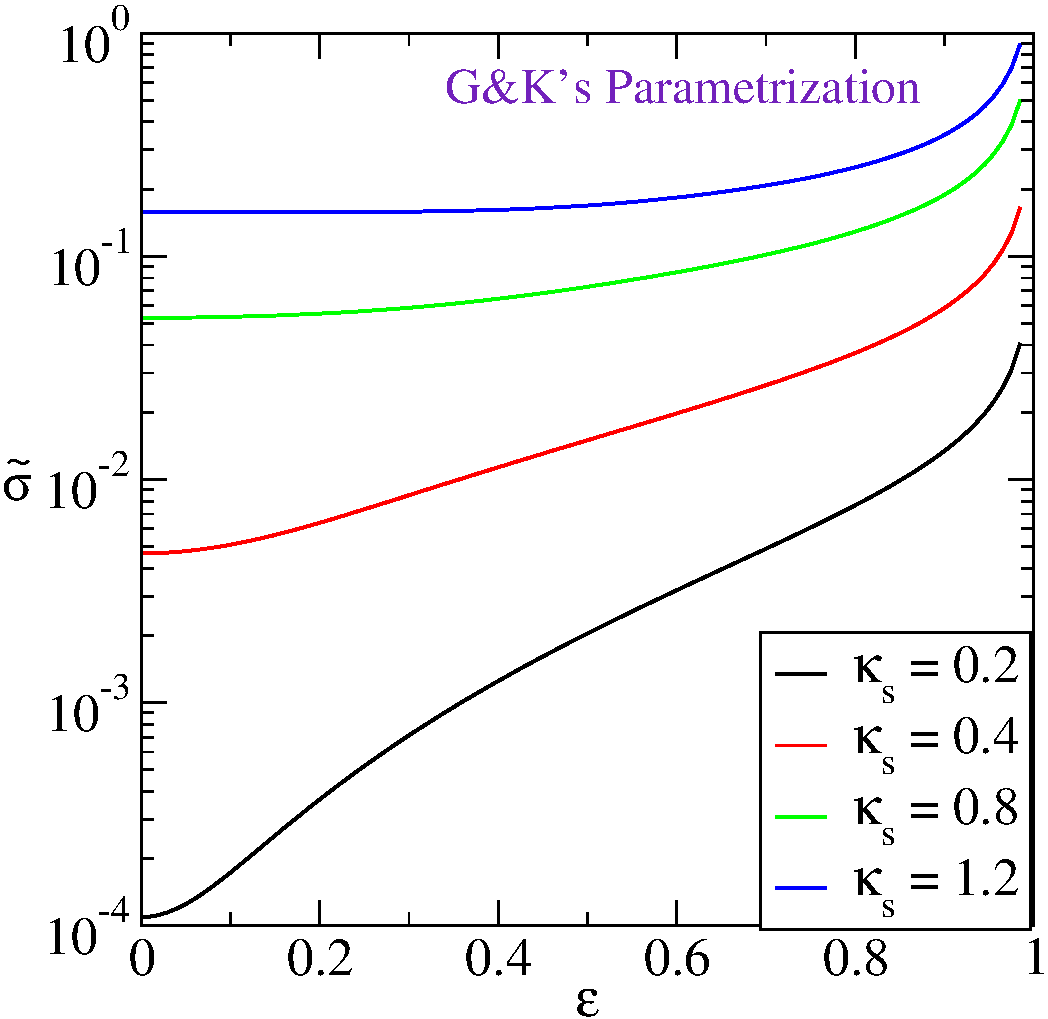
\includegraphics{graphics/dcs_pnfw_vs_e-gk.pdf}}\hspace{1.cm}
\subfigure{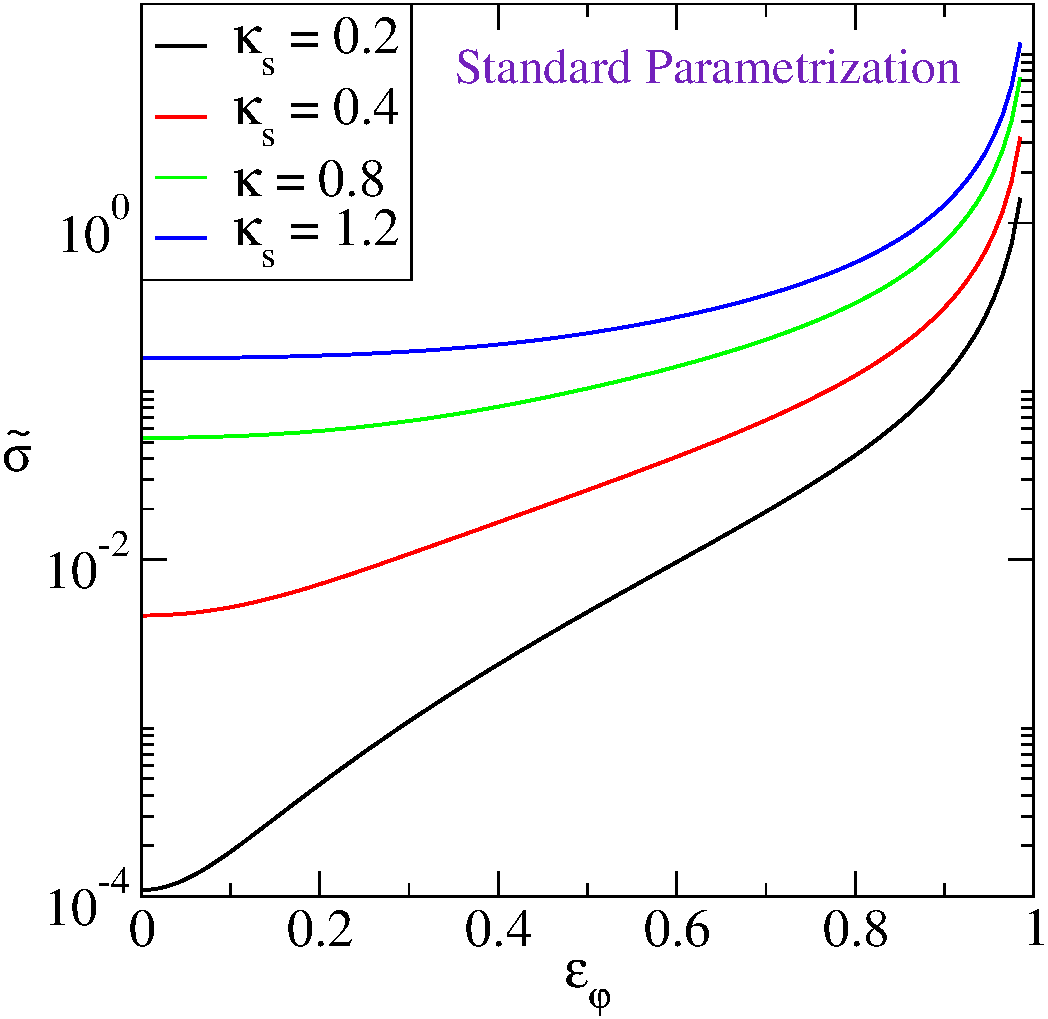
\includegraphics{graphics/dcs_pnfw_vs_e-st.pdf}}\hspace{1.cm}
\subfigure{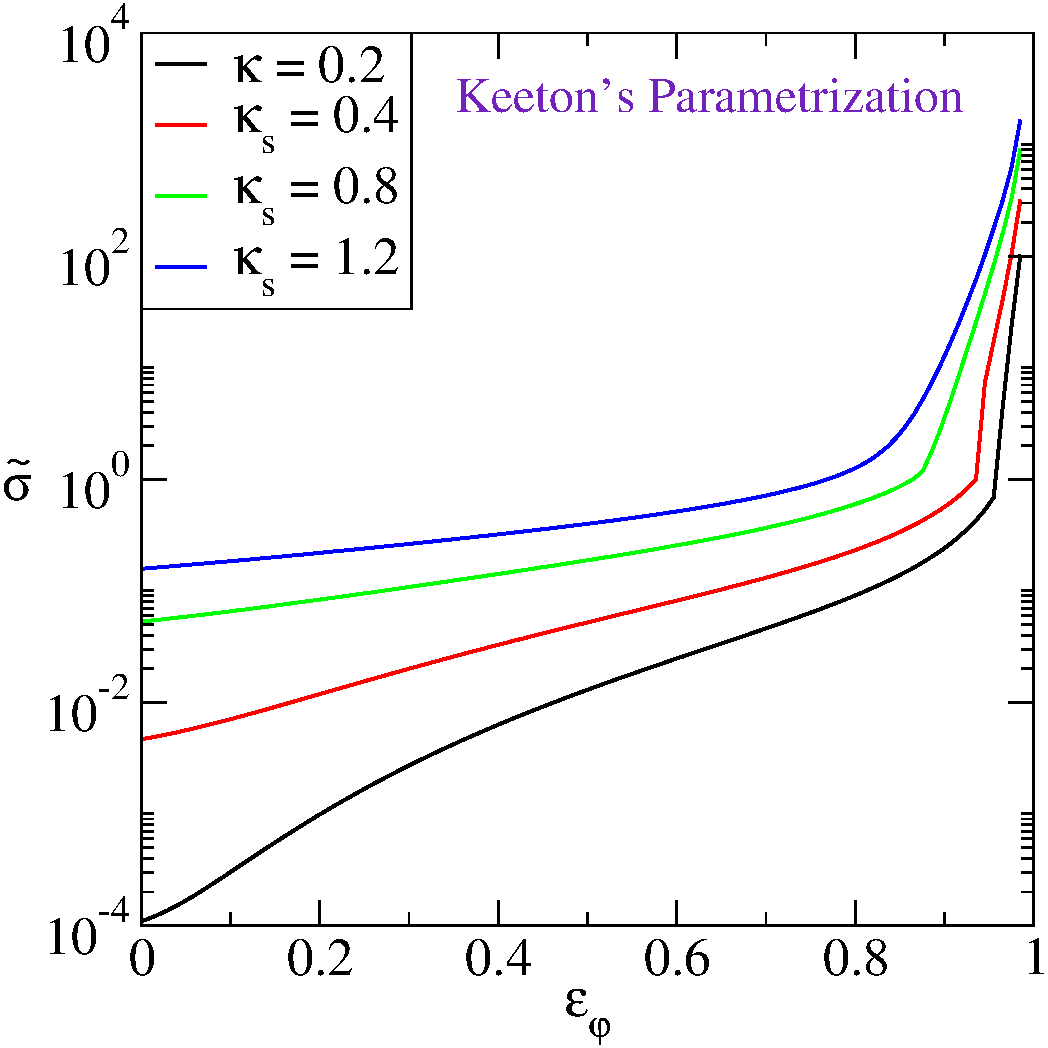
\includegraphics{graphics/dcs_pnfw_vs_e-k.pdf}}}
\caption{\label{dcs_pnfw_e} Deformation cross section for the  PNFW lensing
model as a function of the ellipticity. Left Panel: 
Parametrization of the Angle Deflection Model. Middle Panel: Standard
Parametrization. Right Panel: The Keeton's parametrization. The calculations
were done for $R_{\rm th}=10$ and $r_s=1$.}
\end{figure*}

\begin{figure*}[!ht]
\resizebox{\hsize}{!}{
\subfigure{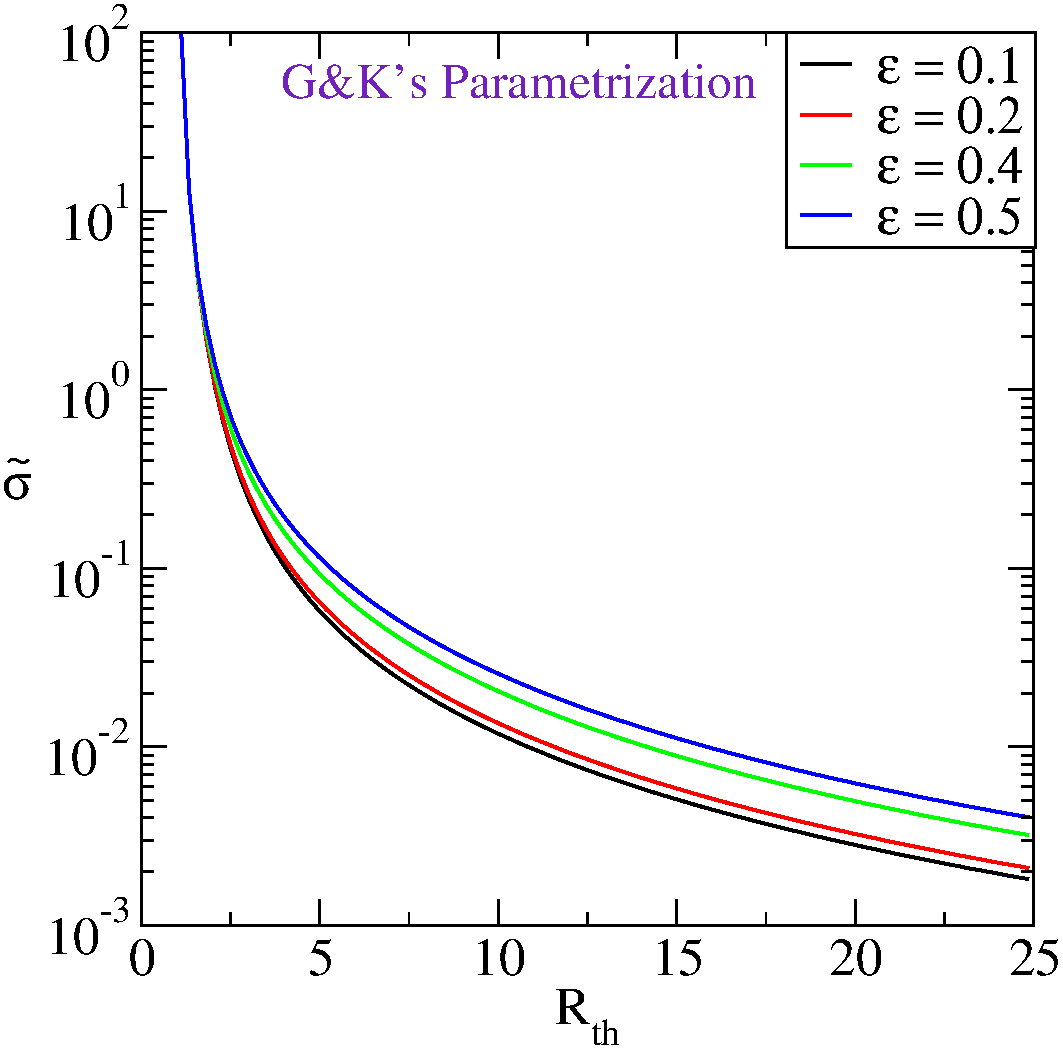
\includegraphics{graphics/dcs_pnfw_vs_rth-gk.pdf}}\hspace{1.cm}
\subfigure{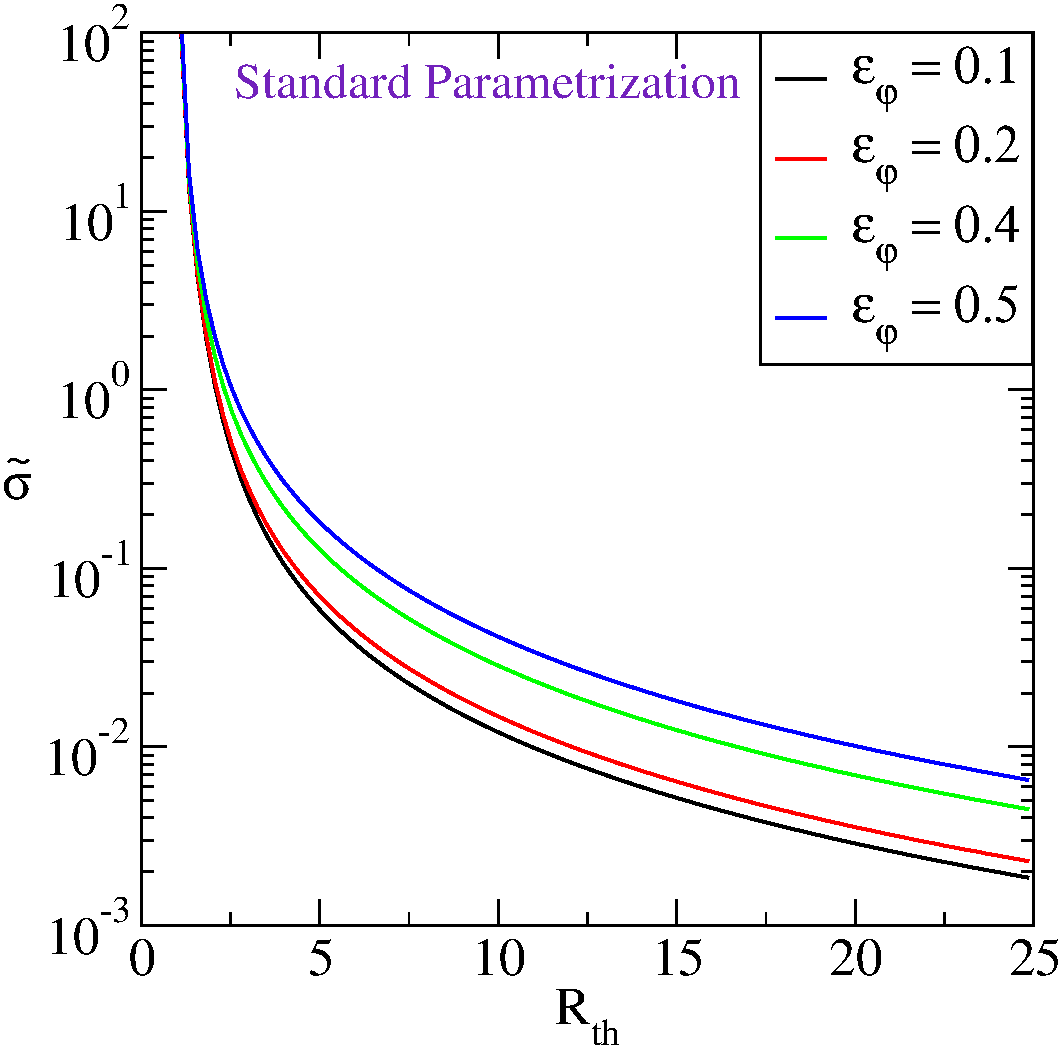
\includegraphics{graphics/dcs_pnfw_vs_rth-st.pdf}}\hspace{1.cm}
\subfigure{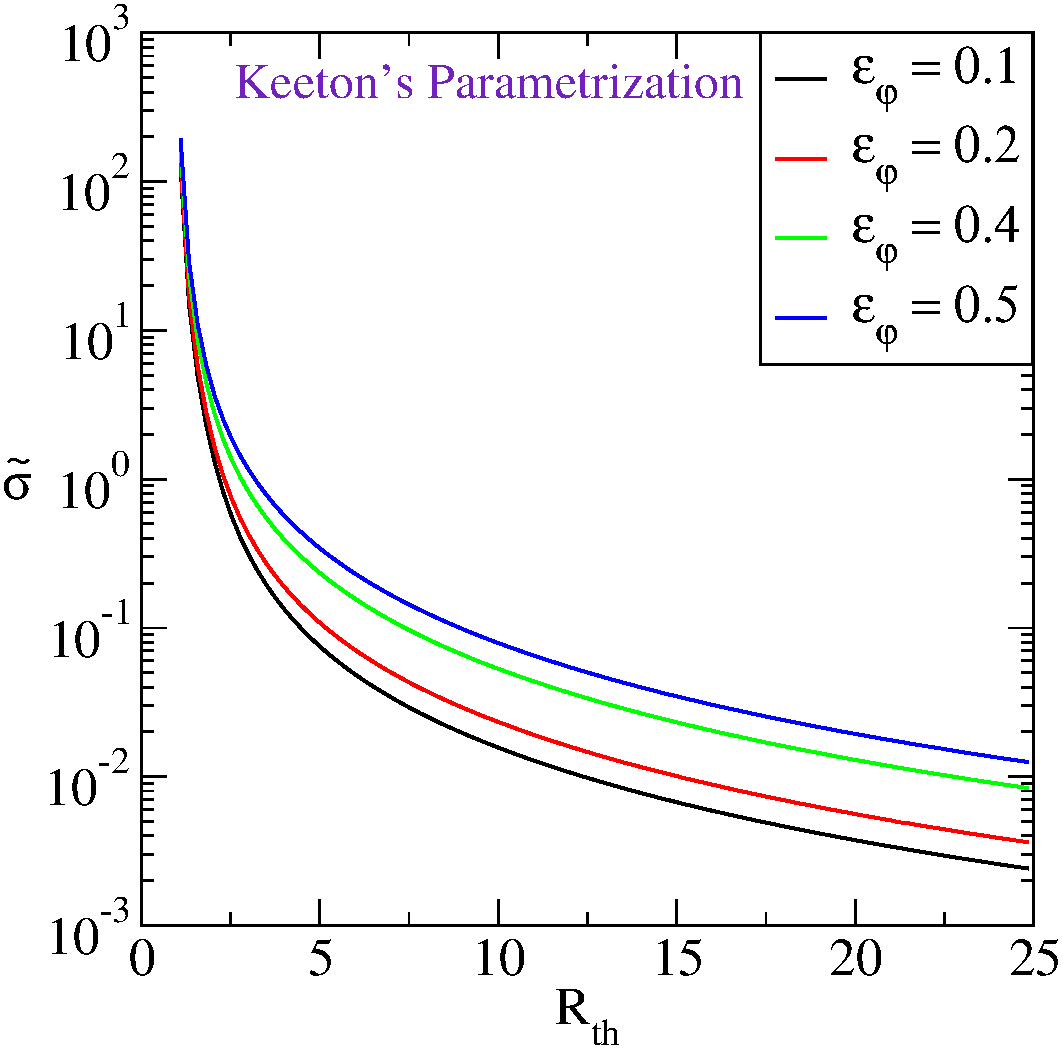
\includegraphics{graphics/dcs_pnfw_vs_rth-k.pdf}}}
\caption{\label{dcs_siep_rth} Deformation cross section for the  PNFW lensing
model as a function of $R_{\rm th}$. Left Panel:
Parametrization of the Angle Deflection Model. Middle Panel: Standard
Parametrization. Right Panel: The Keeton's parametrization. The calculations
were done for $\kappa_s=0.5$ and $r_s=1$.}
\end{figure*}
